\chapter{Basic Covariance Functions}
\label{chapBasicCovarianceKernels}
The \ref{partIncorporatePattern} part of the thesis shows how to incorporate prior information of patterns into building GP models. The chapter \cite{chapBasicCovarianceKernels} shows few basic kernel types, while the chapter \ref{chapCombiningBasicCovariances} shows how to combine these basic kernels together and incorporate more complex patterns. This part \ref{partIncorporatePattern} is heavily inspired from works of \cite{duvenaud-thesis-2014, wilson2014thesis, lloyd2014automatic, durrande2001etude} 

The covariance functions discussed in this chapter are pretty known in the machine learning literature, but unfortunately not often used to build engineering models. The original contribution of chapter \ref{chapBasicCovarianceKernels} is application of basic kernels to build meaningful engineering models. We build a model using spectral mixture kernel (section \ref{}) to automatically identify structural dynamics parameters from a structural experiment \cite{chiplunkar2017operational}. We also apply a change-point kernel (section \ref{}) to detect start of plasticity in a structural experiment and start of separation on an airfoil \cite{chiplunkar:hal-01555401}.  

\textbf{This chapter unfolds as follows}

\section{Properties}\label{secPropertiesOfCovariance}
A kernel is a function that maps any pair of inputs into \(\mathcal{R}\). The covariance of a GP is an example of a kernel, which specifies covariance of a pair of random functions \(f(x_{i})\) and \(f(x_{j})\) situated a points \(x_{i}\) and \(x_{j}\) (mostly written as a function of \(x_{i}\) and \(x_{j}\)). 

Several learning algorithms work on distance measures, i.e. if two points are closer then their observations will also tend to be similar. Covariance functions are methods to specify the measure of distance in GP Regression. If two points have a high value of covariance then, they are similar and hence will have similar value of observations. Therefore, by defining a covariance function we encode biases into our family of functions. Biases based on smoothness (section \ref{}), linearity (section \ref{}), differentiability (section \ref{}) etc can be easily encoded using simple covariance functions.

For a zero mean GPs as specified in section \ref{subSecCH2MeanFunction} a covariance function between \(f(x_{i})\) and \(f(x_{j})\) can be written as equation \ref{eqCovariance}.

\begin{equation}\label{eqCovariance}
    k(x_{i}, x_{j}) = cov(f(x_{i}), f(x_{j}))
\end{equation}

A covariance function \(k(x_{i}, x_{j})\) is always symmetric, since: 

\begin{equation}\label{eqSymmetricCovariance}
    k(x_{i}, x_{j}) = cov(f(x_{i}), f(x_{j})) = cov(f(x_{j}), f(x_{i})) =  k(x_{j}, x_{i})
\end{equation}

A covariance is function is a Positive Semi Definite (PSD) function, consider for a new random vector \(T = \sum \alpha_{i}f(x_{i})\):

\begin{equation}\label{eqDerivePSDCovariance}
    \begin{aligned}
        var(T) & = cov\left ( \sum_{i} \alpha_{i}f(x_{i}), \sum_{j} \alpha_{j}f(x_{j}) \right ) = \sum_{i}\sum_{j}\alpha_{i}\alpha_{j}cov(f(x_{i}), f(x_{j})) \\
& = \sum_{i}\sum_{j}\alpha_{i}\alpha_{j}k(x_{i}, x_{j})
    \end{aligned}
\end{equation}

Since a variance is positive, hence:
\begin{equation}\label{eqPSDCovariance}
\sum_{i}\sum_{j}\alpha_{i}\alpha_{j}k(x_{i}, x_{j}) \geq 0
\end{equation}

In fact \(k(x_{i}, x_{j})\) corresponds to a covariance function iff it is a symmetric PSD function \cite{loeve1978probability, durrande2001etude}. The positive definite requirement means that the covariance kernel corresponds to an inner product in some basis space \cite{bishop2006pattern}. A Gram matrix constructed from a PSD function is a PSD matrix, checking if a matrix is PSD is simple and implemented in several software packages. A cholesky decomposition only exists for a Gram matrix constructed from a PSD function\footnote{Remember cholesky decomposition is also called the square root of a matrix, square root only exists for positive numbers}. 

After accounting for the zero mean, the GP model can be completely parametrized by the kernel. Hence the problem of learning in a Gaussian Process is exactly the problem of finding suitable properties of the covariance function \cite{rasmussen2006gaussian}. The covariance function consists of two parts a functional form (which define a pattern for constituent family of functions) and a set of hyper-parameters (which define the probability distribution for constituent family of functions). In section \ref{} we have seen in detail how to automatically choose hyper-parameters. The current chapter and the next chapter will detail how to choose the functional form. Although there exist methods in the literature to automatically choose the functional form of a covariance function \cite{duvenaud-thesis-2014, lloyd2014automatic, automaticStatistician}, we will not detail those methods here. 

\section{Bayesian Linear Regression}




Section \ref{sec:covStructure} will show commonly used covariance functions and how to combine them for introducing structure in the model. Section \ref{sec:multiOutputKernels} deals with how to merge multiple outputs in a single kernel for making a better model.

\section{Expressing Structure with Kernels} \label{sec:covStructure}
Neural networks initially became popular because they could automatically detect hidden pattern in data. Gaussian Process are effectively smoothing devices, if used with a proper kernel (squared exponential). Simple kernels cannot discover structure in the data and cannot extrapolate. This observation prompted MacKay \cite{mackay2003information} to ask the question "Have we thrown the baby out with the bathwater?" in replacing Gaussian Process with Neural Networks. This section will show how to encode different types of structure in a kernel and eventually how to progressively combine them to discover understandable structure in data \cite{duvenaud-thesis-2014}.



\subsection{Squared Exponential Kernel}
The Squared Exponential (SE) kernel, also called radial basis function or exponentiated quadratic kernel, is the most widely used kernel. This is probably because it defines a hypothesis space of all highly smooth functions while having only two parameters section: \ref{sec:GaussianProcess}.

\begin{equation}
k_{\textrm{SE}}(x, x') = \sigma^2\exp\left(-\frac{(x - x')^2}{2\ell^2}\right)
\end{equation}

The length-scale $l$ determines the wiggliness of the functions in the hypothesis space, generally one cannot extrapolate more than $l$ units away from your data. The output variance $\sigma^{2}$ determines the amplitude of the functions. Fig: \ref{subfig:SEDraws} shows random draws from the hypothesis space of SE kernel with hyperpameters $l = 0.2$  and  $\sigma = 1$

\subsection{Mat\'ern Kernel}\label{subsec:maternKernel}
The Mat\'ern kernel is the second most popular kernel after the squared exponential. Researchers argue that the highly smooth assumption of the squared exponential function is unrealistic in several cases \cite{stein2012interpolation}. Mat\'ern kernel provides the flexibility to define a hypothesis space of functions with varying degree of derivability. 

\begin{align}
k_{Matern}(x, x') = \frac{2^{1- \nu }}{\Gamma (\nu)}\left ( \frac{\sqrt{2\nu(x-x'))}}{l} \right )^{\nu}K_{\nu}\left ( \frac{\sqrt{2\nu(x-x'))}}{l} \right)
\end{align}

$\nu$ defines the derivability of the functions in the hypothesis space. The most interesting cases for machine learning are when $\nu = 3/2$ or $\nu = 5/2$ since they define functions which are derivable once or twice \cite{rasmussen2006gaussian}. Fig: \ref{subfig:matern3Draws} shows random draws from a Mat\'ern kernel with the hyperparameters $\nu = 3/2$, $l = 0.2$ and  $\sigma = 1$. 

Mat\'ern kernels have been found to have superior performance on datasets with high-dimensions \cite{le2013fastfood}. It is argued that the Mat\'ern kernel accounts for the concentration of measure effect in higher-dimensions. Imagine a high-dimensional orange (it is tough to imagine more than 3 dimensions), but if there was a high dimensional orange than most of its mass will be concentrated in its skin and not its pulp \cite{domingos2012few}. This causes issues in concept of distance in higher dimensions, since learning algorithms use similarity measures (or some measure of distance) several learning algorithm suffer from the problem of concentration of measure effect.

In our experiments the Mat\'ern kernel performs significantly well when compared to SE kernels. This improved performance is due to the increased hypothesis space or better performance in higher dimensions should be a matter of study.

\subsection{Linear Kernel} 
A linear kernel represents a hypothesis space on linear functions. Using a linear kernel means we are effectively performing Bayesian Linear Regression. Linear kernel when combined with other kernels brings about some very nice properties discussed in subsection \ref{subsec:structureKernelsMultiplyingKernels}.

\begin{align}
k_{\textrm{Lin}}(x, x') = \sigma_v^2(x - c)(x' - c)
\end{align}

The linear kernel is not like other kernels it is non-stationary. Stationary kernels are generally a function of $(x-x')$. This gives stationary kernels a nice property that they are irrelevant to displacing the data points. Fig: \ref{subfig:linearDraws} shows random draws from a Linear kernel.

\subsection{Change-Point kernels}
Changepoint (CP) kernels can be defined through addition and multiplication with sigmoidal functions. They were introduced to identify changepoints in time-series modelling \cite{osborne2010bayesian}. This kernel expresses a change from one structure to another. 

\begin{align} \label{eq:changePointKernel}
CP(k_{1}, k_{2}(x, x')) = sigm(x)k_{1}sigm(x') + (1-sigm(x))k_{2}(1-sigm(x'))
\end{align}

The parameters of the sigmoidal determine the steepness of the changepoint and the placement of changepoint.

\subsection*{Identifying physical parameters using CP kernel}\label{subsubsec:applicationCP}
In several physical processes, there is an equilibrium condition. Near this equilibrium, a linear approximation is performed and when the assumptions start failing a non-linear domain is observed. This basic approximation is made in experiments such as: lift vs alpha curves; estimation of Young's Modulus; basics of control theory. The value of these physical parameters slope (eg. Young's Modulus) and position of changepoint (eg. plasticity) are progressively fed into further simulations. 

These basic physical properties define the general characteristics of the field. The parameters are then later fed into more complex designs and used as an input into particular mesh elements (remember induction vs deduction \ref{sec:machineLearning}). The values of slopes and position of change-point are approximated by engineering judgement. 

\begin{figure}[!ht]
  \centering
    \subfigure[GP regression using a SE kernel]
	    {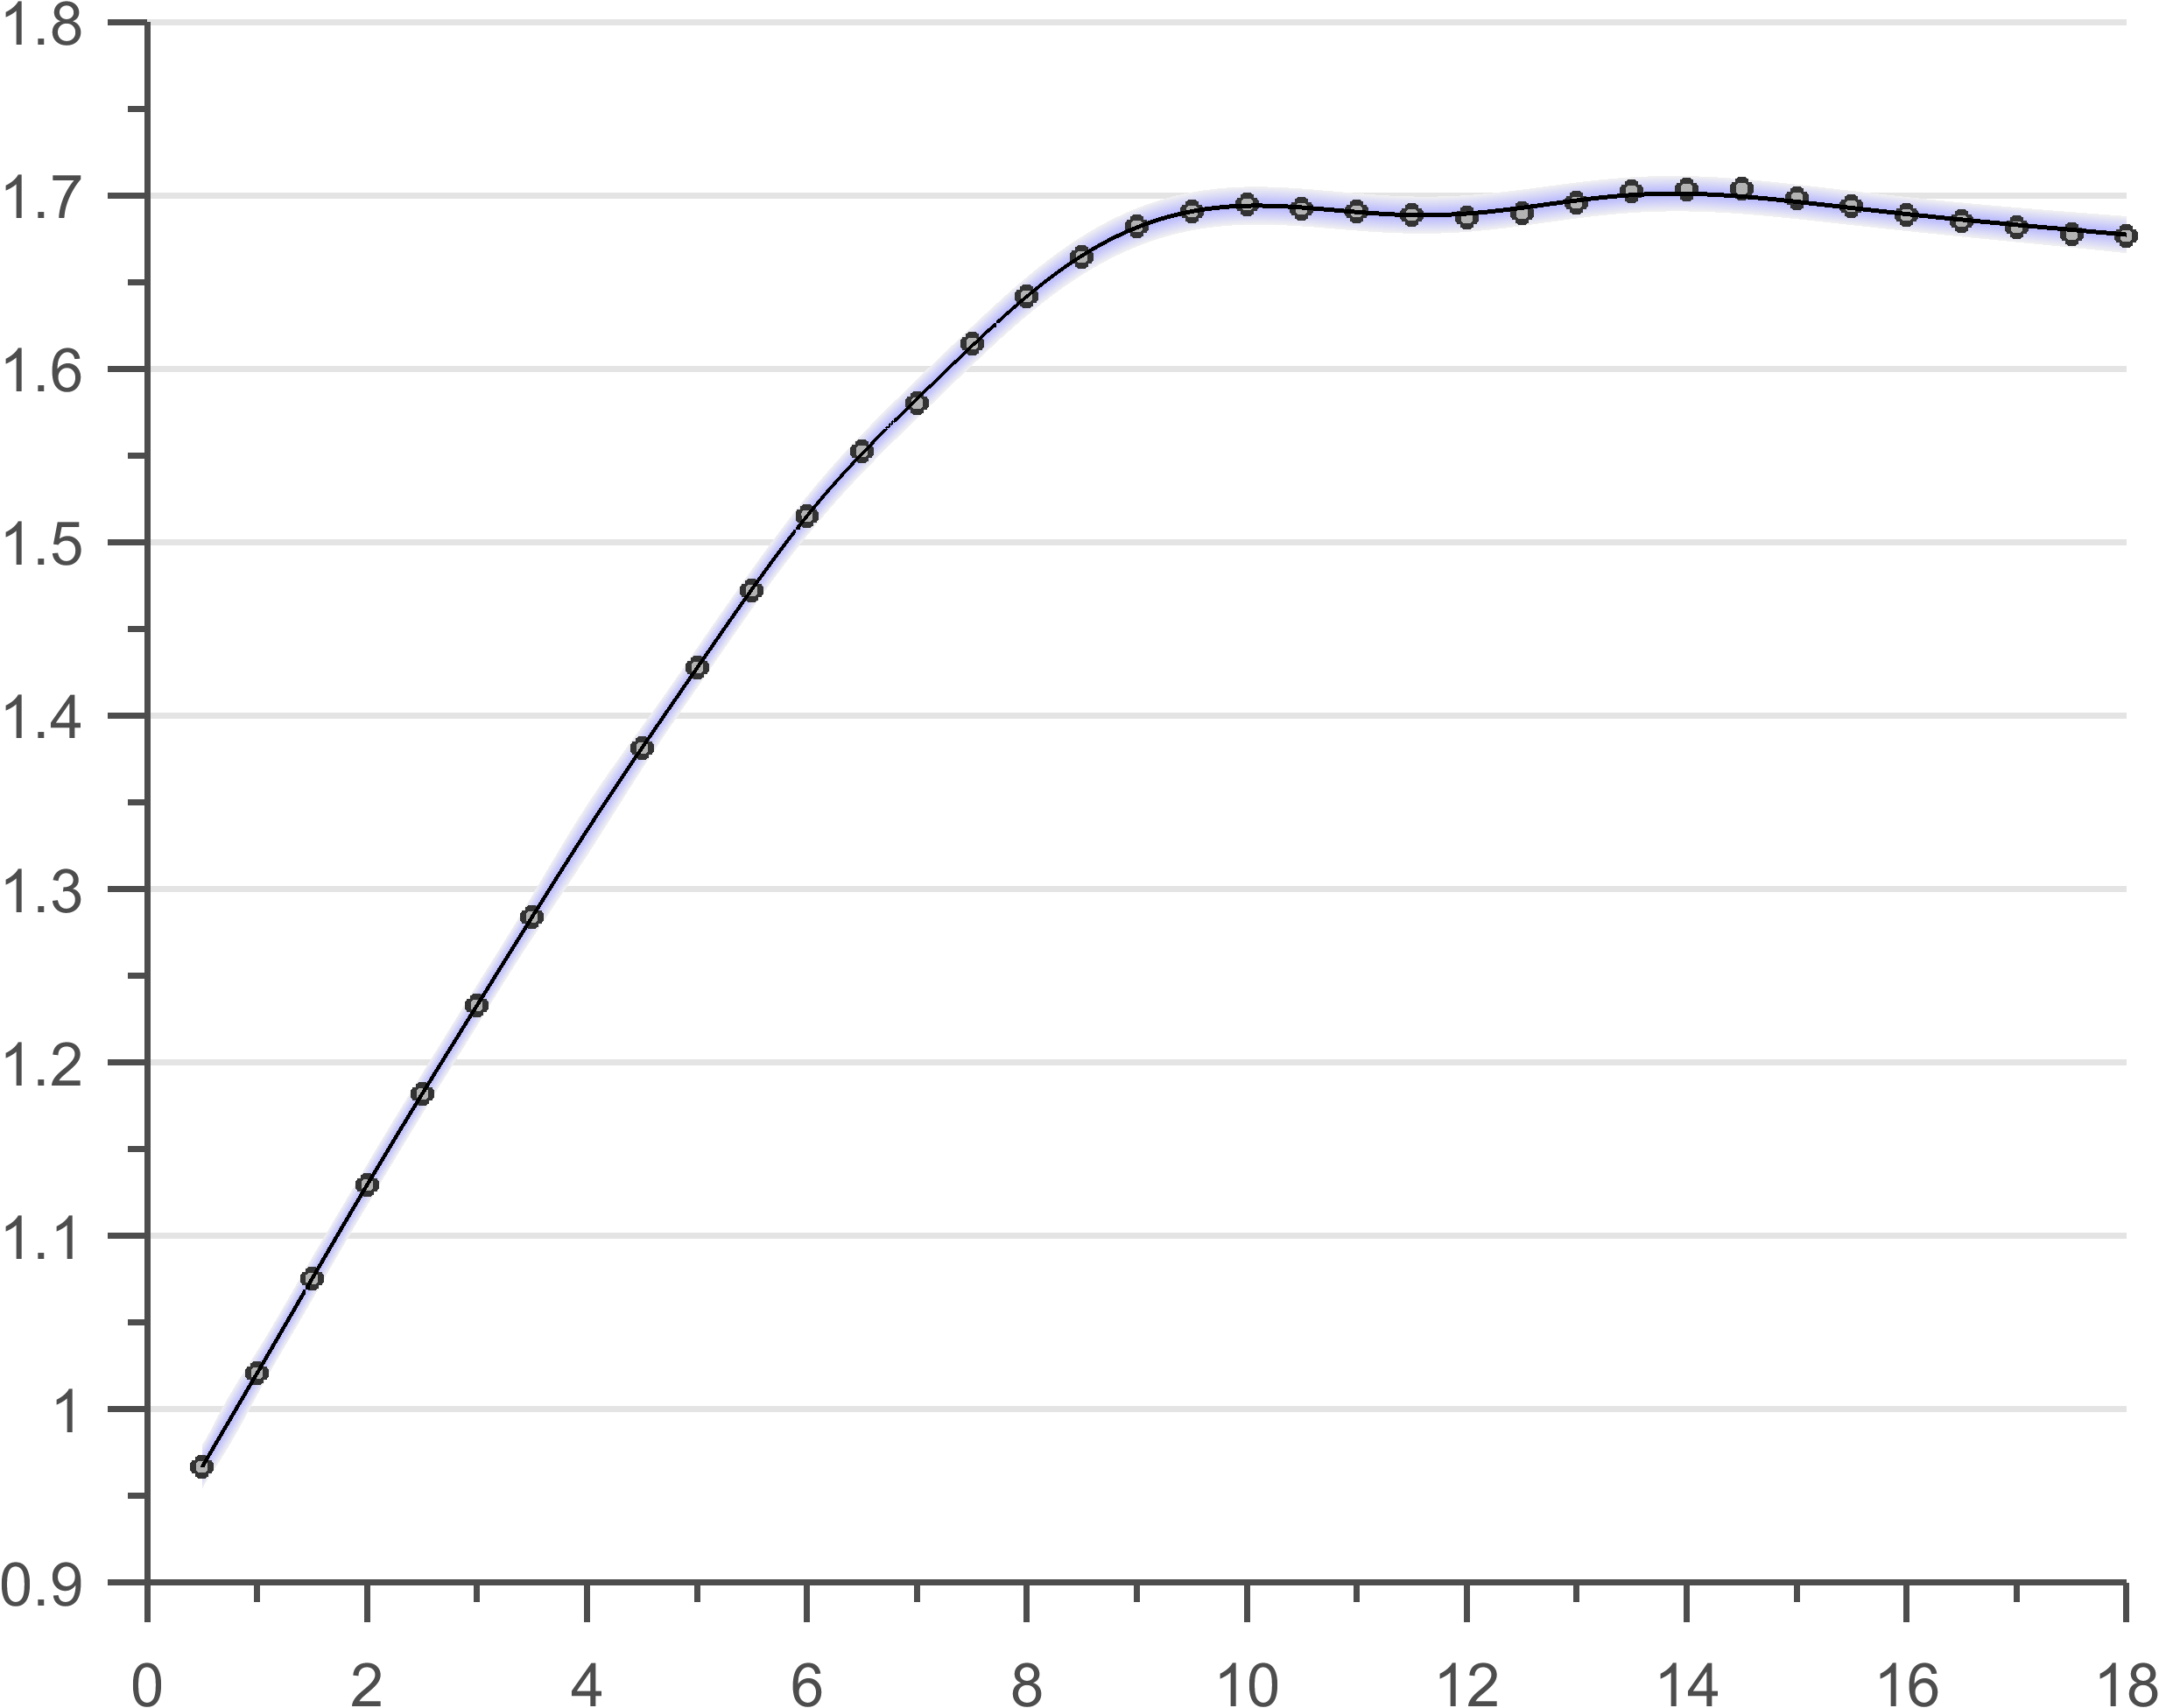
\includegraphics[width=0.45\textwidth]{images/clAlphaCovSE}
	    \label{subfig:clAlphaCovSE}}
	    \quad
    \subfigure[GP regression using a CP(linear, SE) kernel]
	    {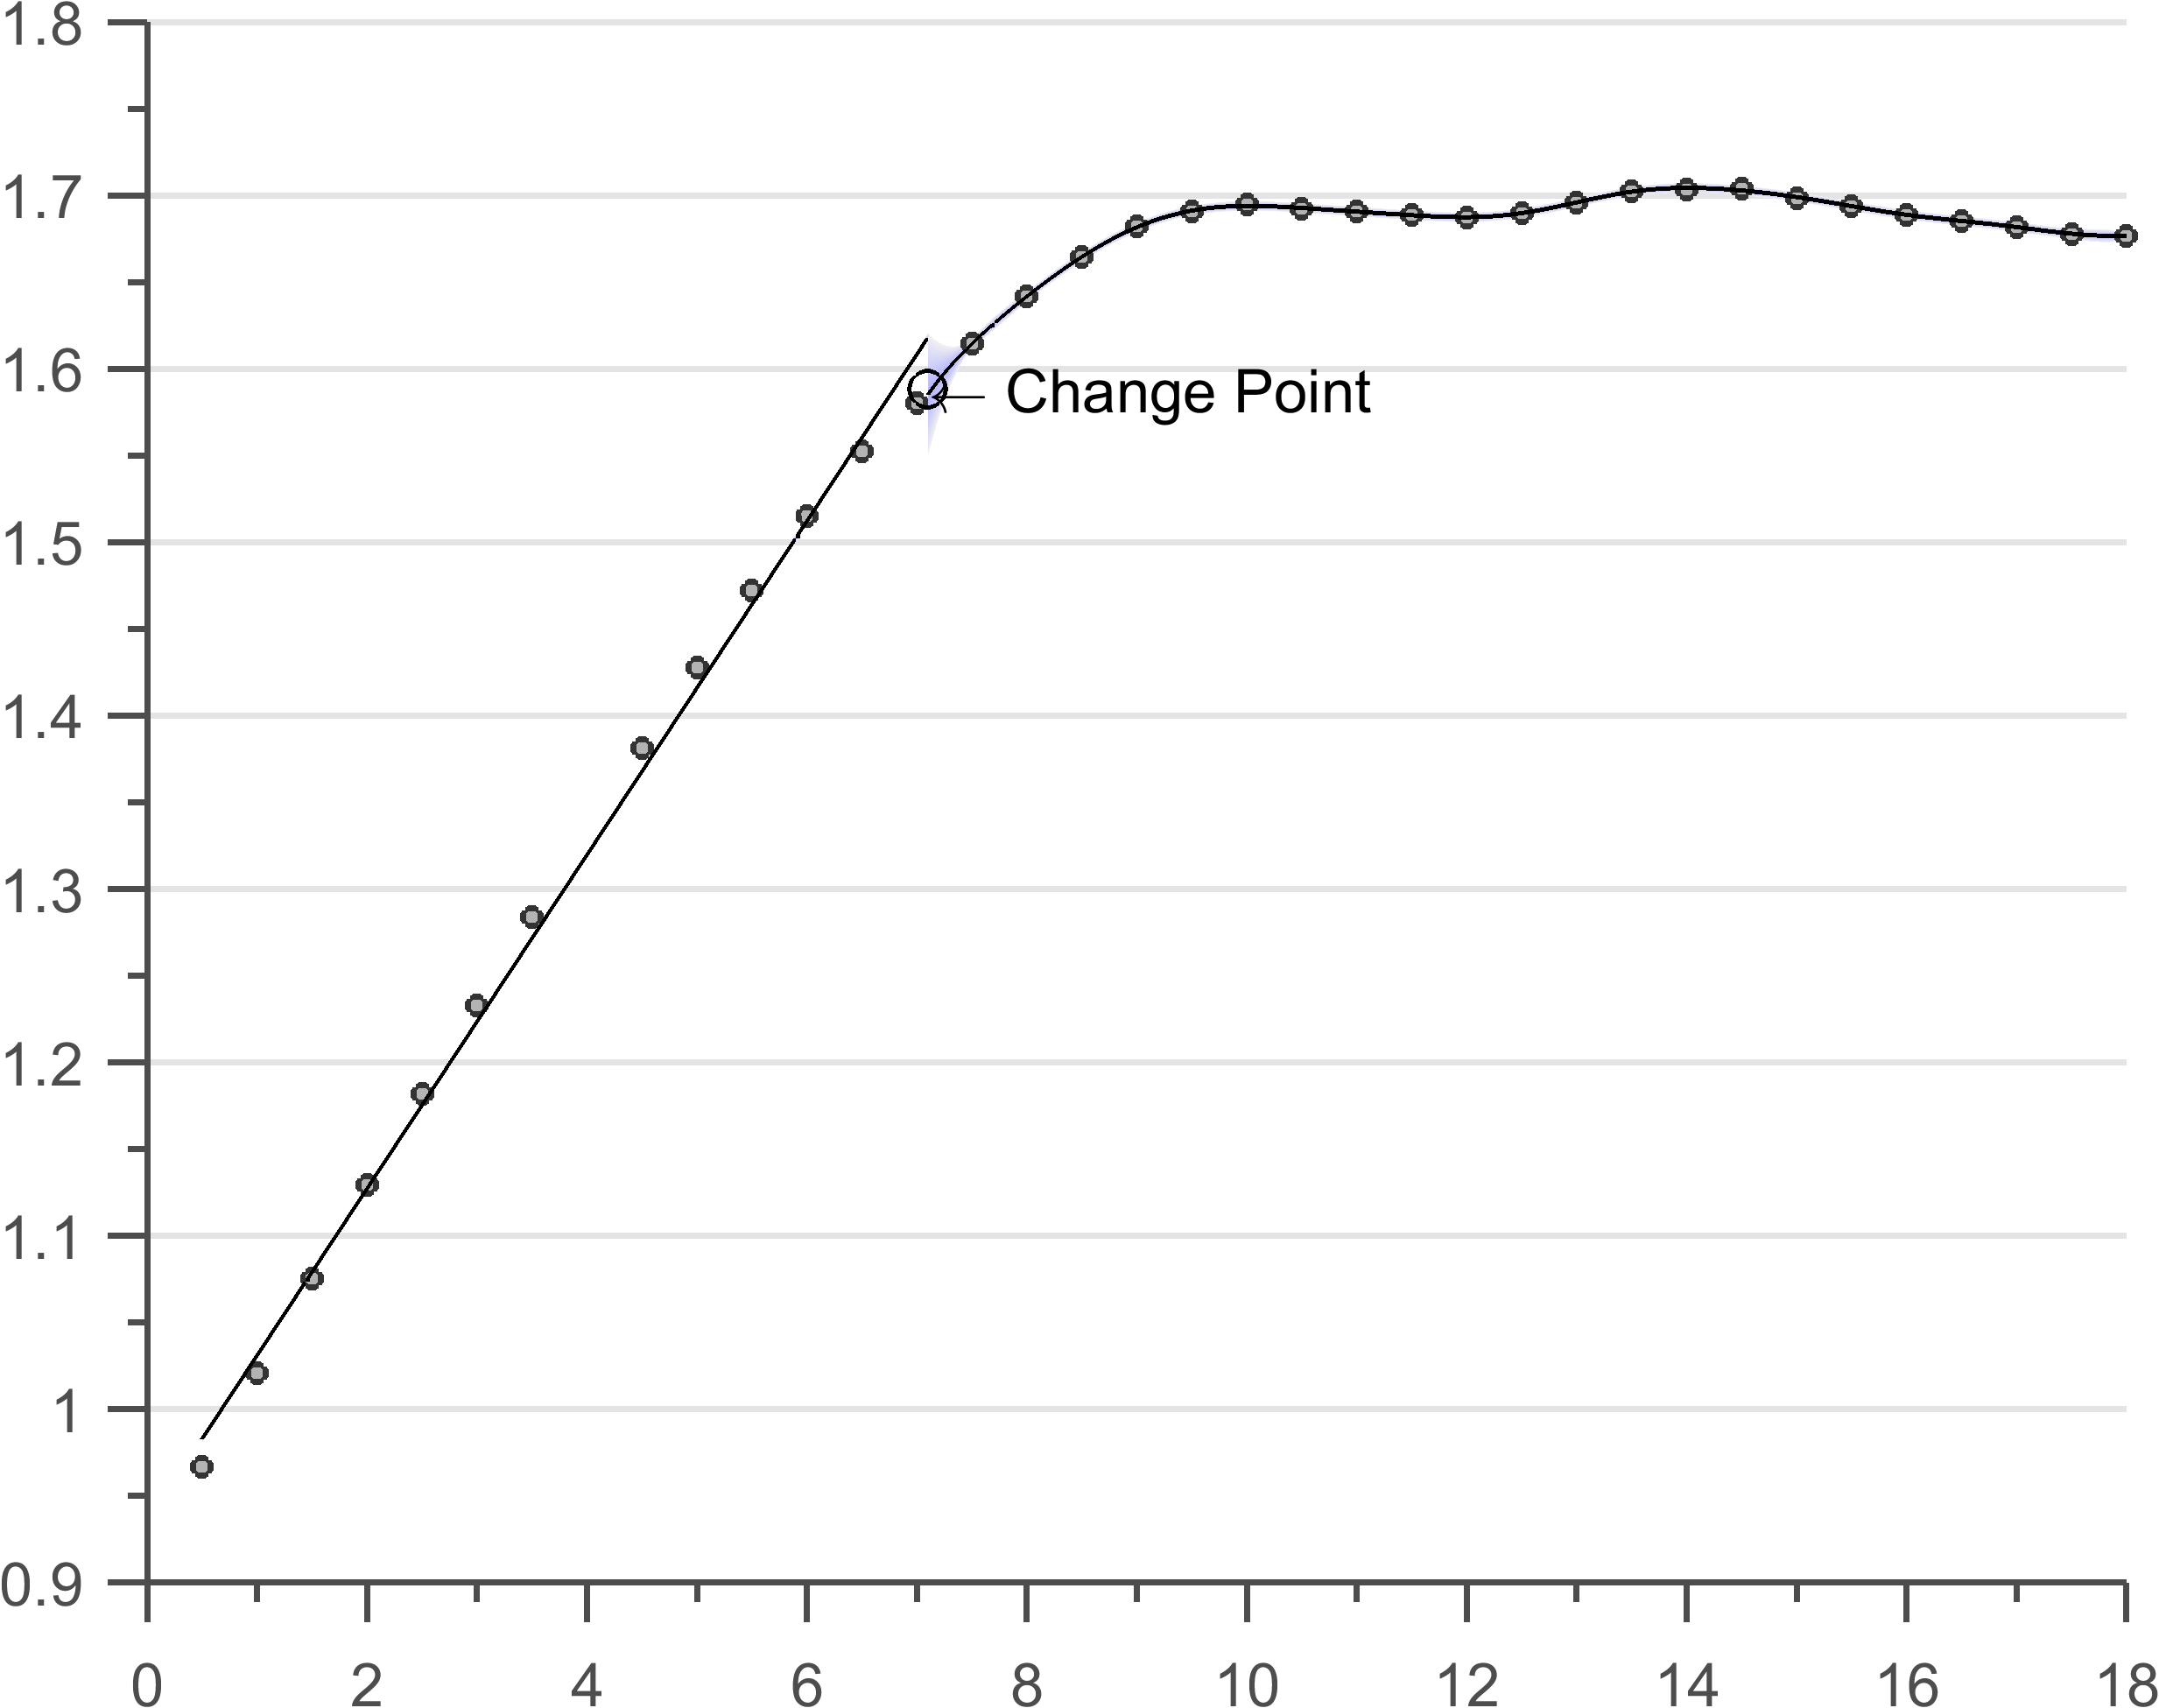
\includegraphics[width=0.45\textwidth]{images/clAlphaCovCP}
	    \label{subfig:clAlphaCovCP}}
	    \caption{Estimation of lift coefficient $Cl\alpha$}
\end{figure}


We tried to solve the problem of estimating the lift coefficient using Gaussian Process. Using the changepoint kernel which transitions from linear domain (linear kernel) to non-linear domain (SE kernel), prior assumptions of the problem were encoded in the kernel structure. Open source data for the lift vs alpha curves for the NACA 0012 airfoil were chosen. Fig: \ref{subfig:clAlphaCovSE} shows the regression of the data using SE kernel. Fig: \ref{subfig:clAlphaCovCP} regression of the same dataset using the CP(linear, SE) kernel. 

We can observe that the algorithm predicts a changepoint for the dataset. This is the point with where the linear assumptions start failing, according to prior information. The marginal likelihood of CP(linear, SE) kernel is rigged with many local minimas. The algorithm tries to put a changepoint at every observation point. Hence using a global optimizer is advised. The changepoint kernel is also very numerically unstable hence cross-validating the learners is also very important (model ensembles \ref{subsec:modelEnsembles}). The results of this study will be presented in the SIAM Uncertainty Quantification 2016 Conference.

\subsection{Spectral Mixture Kernel}
Spectral mixture kernels expand the hypothesis space by exploiting the Bochner's theorem \cite{bochner1959lectures}. It defines a scale-location mixture of finite Gaussian's in the frequency domain \cite{wilson2013gaussian}. 

\begin{align}
k_{\textrm{SM}}(x, x') = \sum_{q=1}^{Q}w_{q}cos(2\pi\mu_{q}^{T}\tau)\prod_{p=1}^{P}exp(-2\pi^{2}\tau_{p}^{2}\nu_{p})
\end{align}

In the frequency domain: the $\mu$ corresponds to modal frequencies; the $\nu$ correspond to damping values and the $w$ corresponds to amplitude or weights of individual gaussians. The Spectral Mixture kernel performs surprisingly well in pattern discovery and extrapolation tasks. But, it falls in the similar trade-off of bias vs variance \ref{subsec:biasVsVariance}. In our experiments the Spectral Mixture kernel performs significantly well in time-series tasks.

\subsubsection{Identifying structural modal parameters using Spectral Mixture Kernel}
Modal analysis has been widely used as a means of identifying dynamic properties such as modal frequencies, damping ratios and mode shapes of a structural system. Traditionally, the system is subjected to artificial input excitations and output deformations (displacements, velocities or accelerations) are measured. These later help in identifying the modal parameters of the system, this process is called Experimental Modal Analysis (EMA). 

Since the last decade Operational Modal Analysis (OMA) has gained considerable interest in the community. OMA identifies the modal parameters only from the output measurements while assuming ambient excitations as random noise. OMA is cheaper because it does not require expensive experimental setup and and can be used in real time operational use cases such as health monitoring \cite{peeters2005industrial} \cite{shahdin2010correlating} \cite{rainieri2007automated}. Several algorithms in OMA can be seen as extensions of EMA algorithms based on the similar assumption of second order MDOF system.

\begin{figure*}[!ht]
  \centering
  \subfigure[Measured output on accelerometers \(x(t)\)]
  {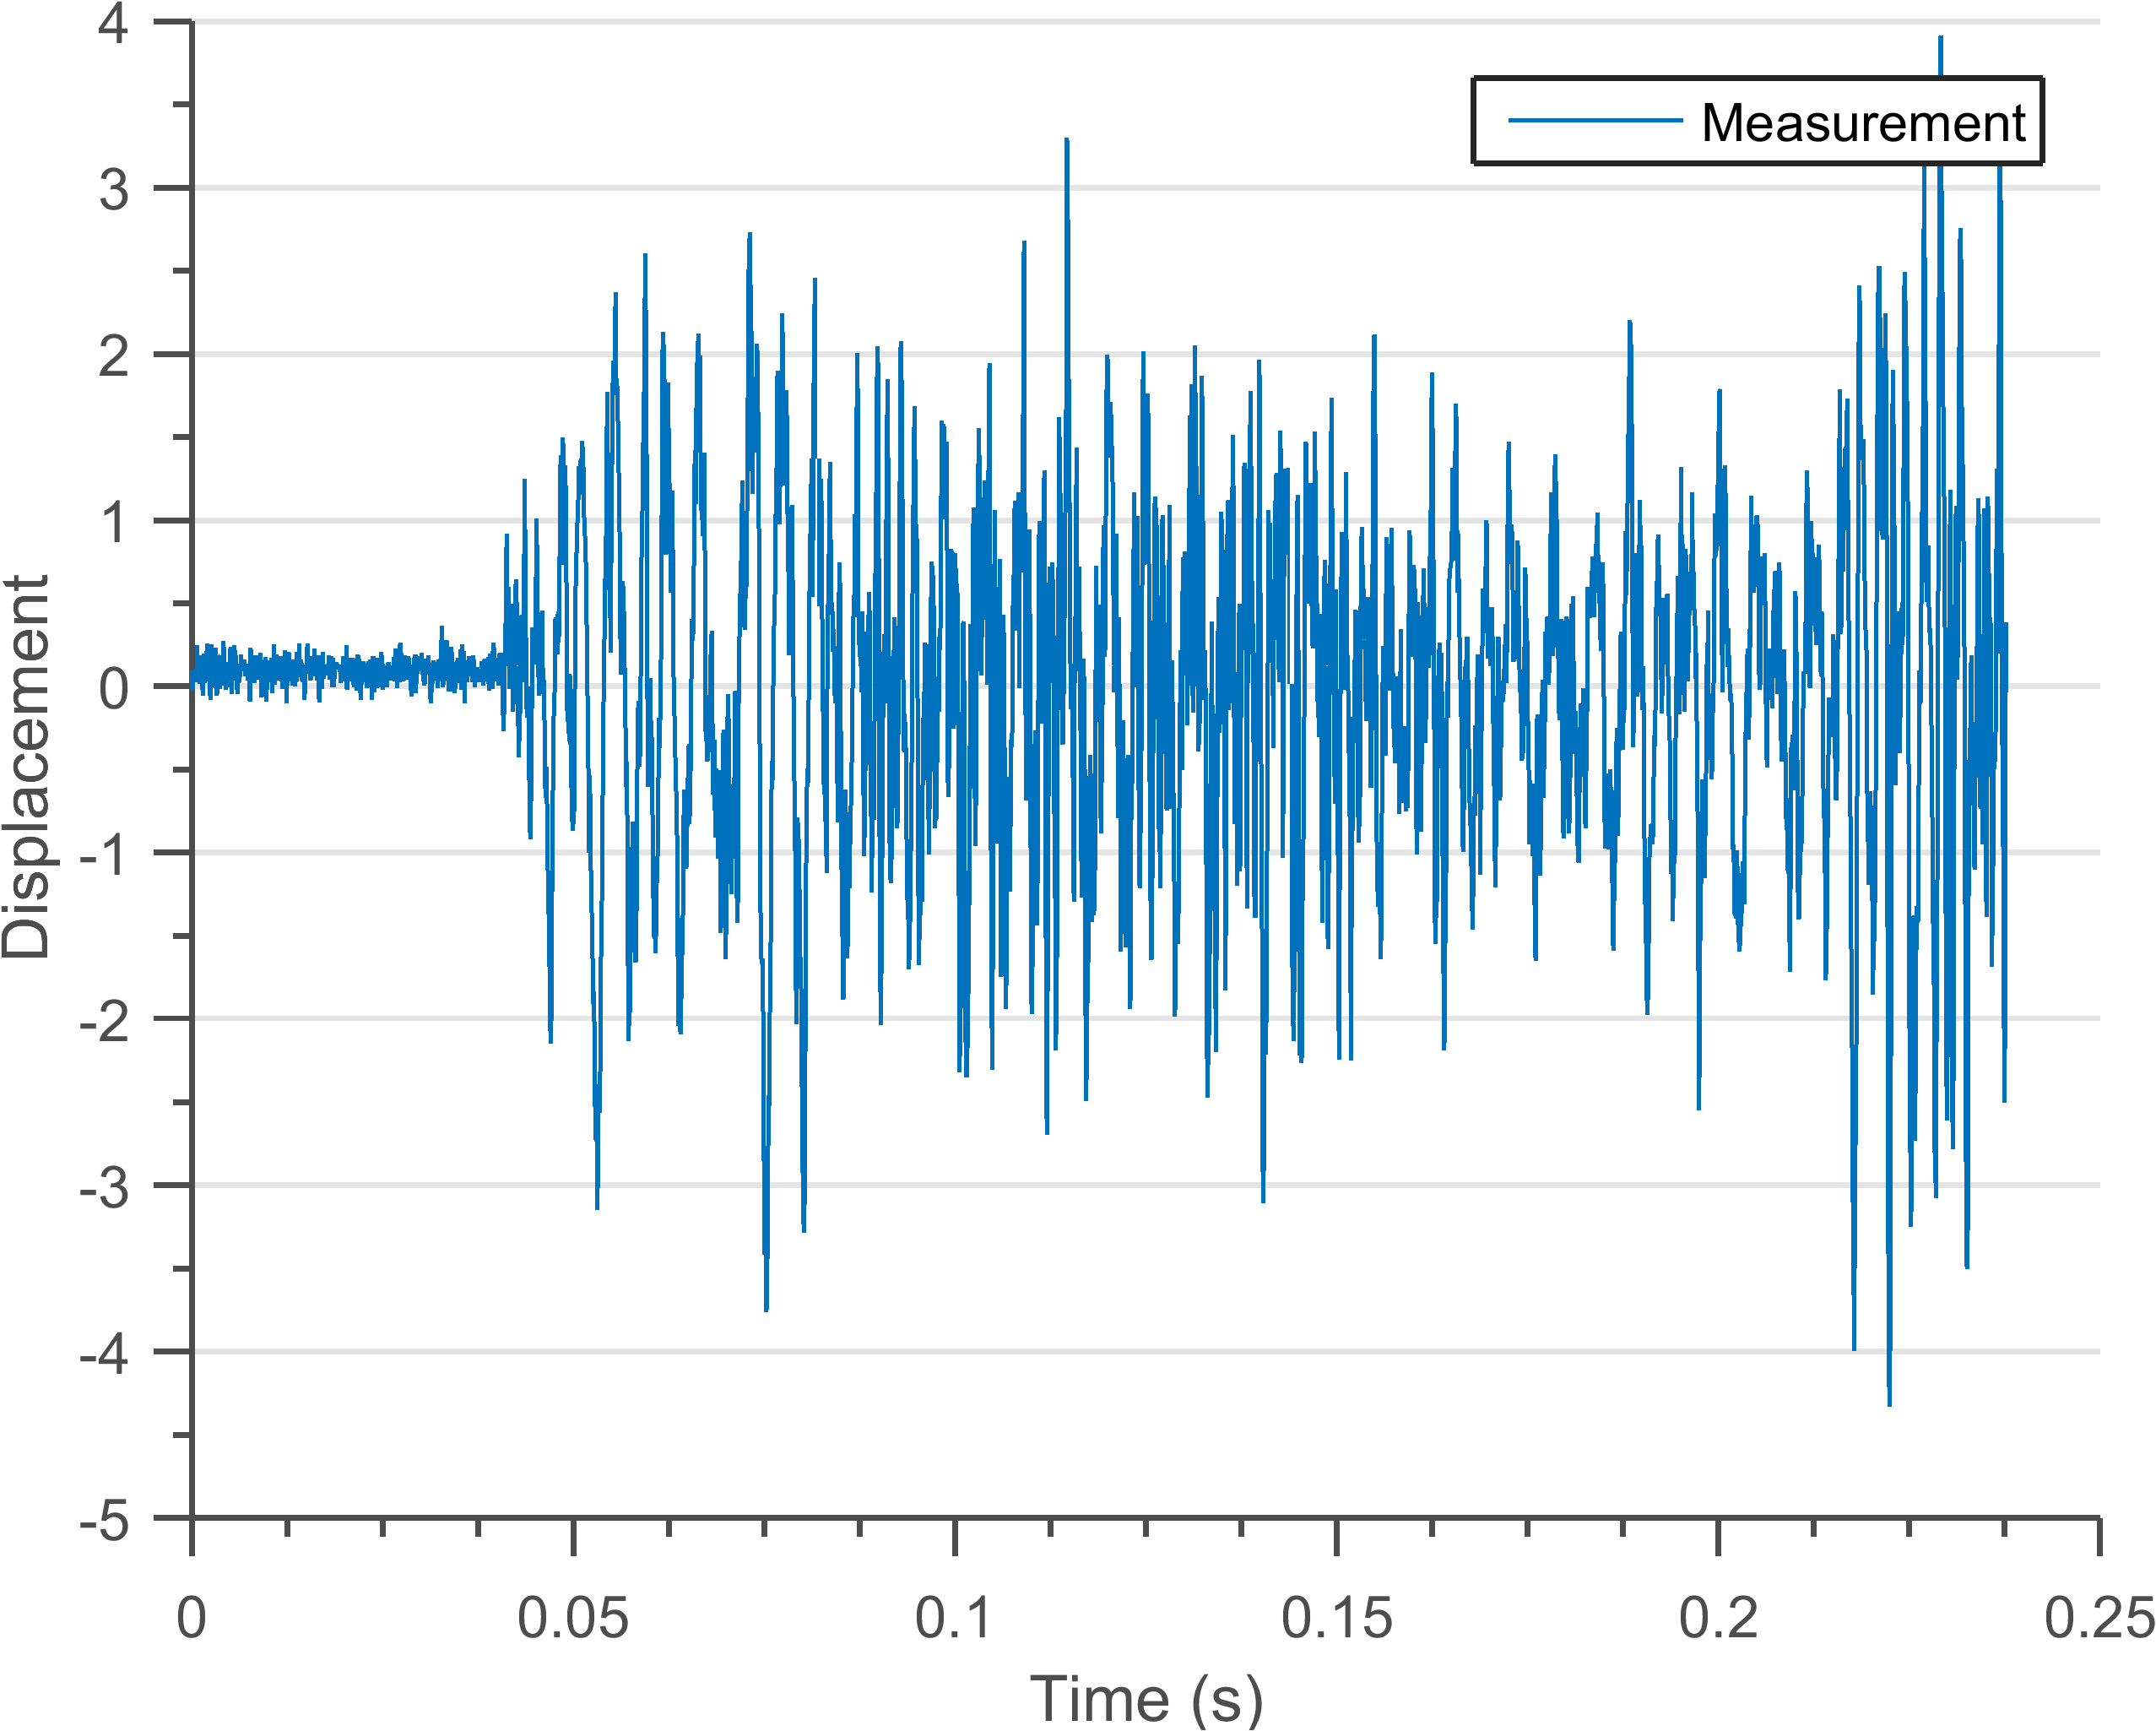
\includegraphics[width=0.3\textwidth]{images/randomOutput}\label{subfig:randomOutput}}\quad
  \subfigure[Auto-correlation \(k(\tau)\) of the measured output fig: \ref{subfig:randomOutput}]
  {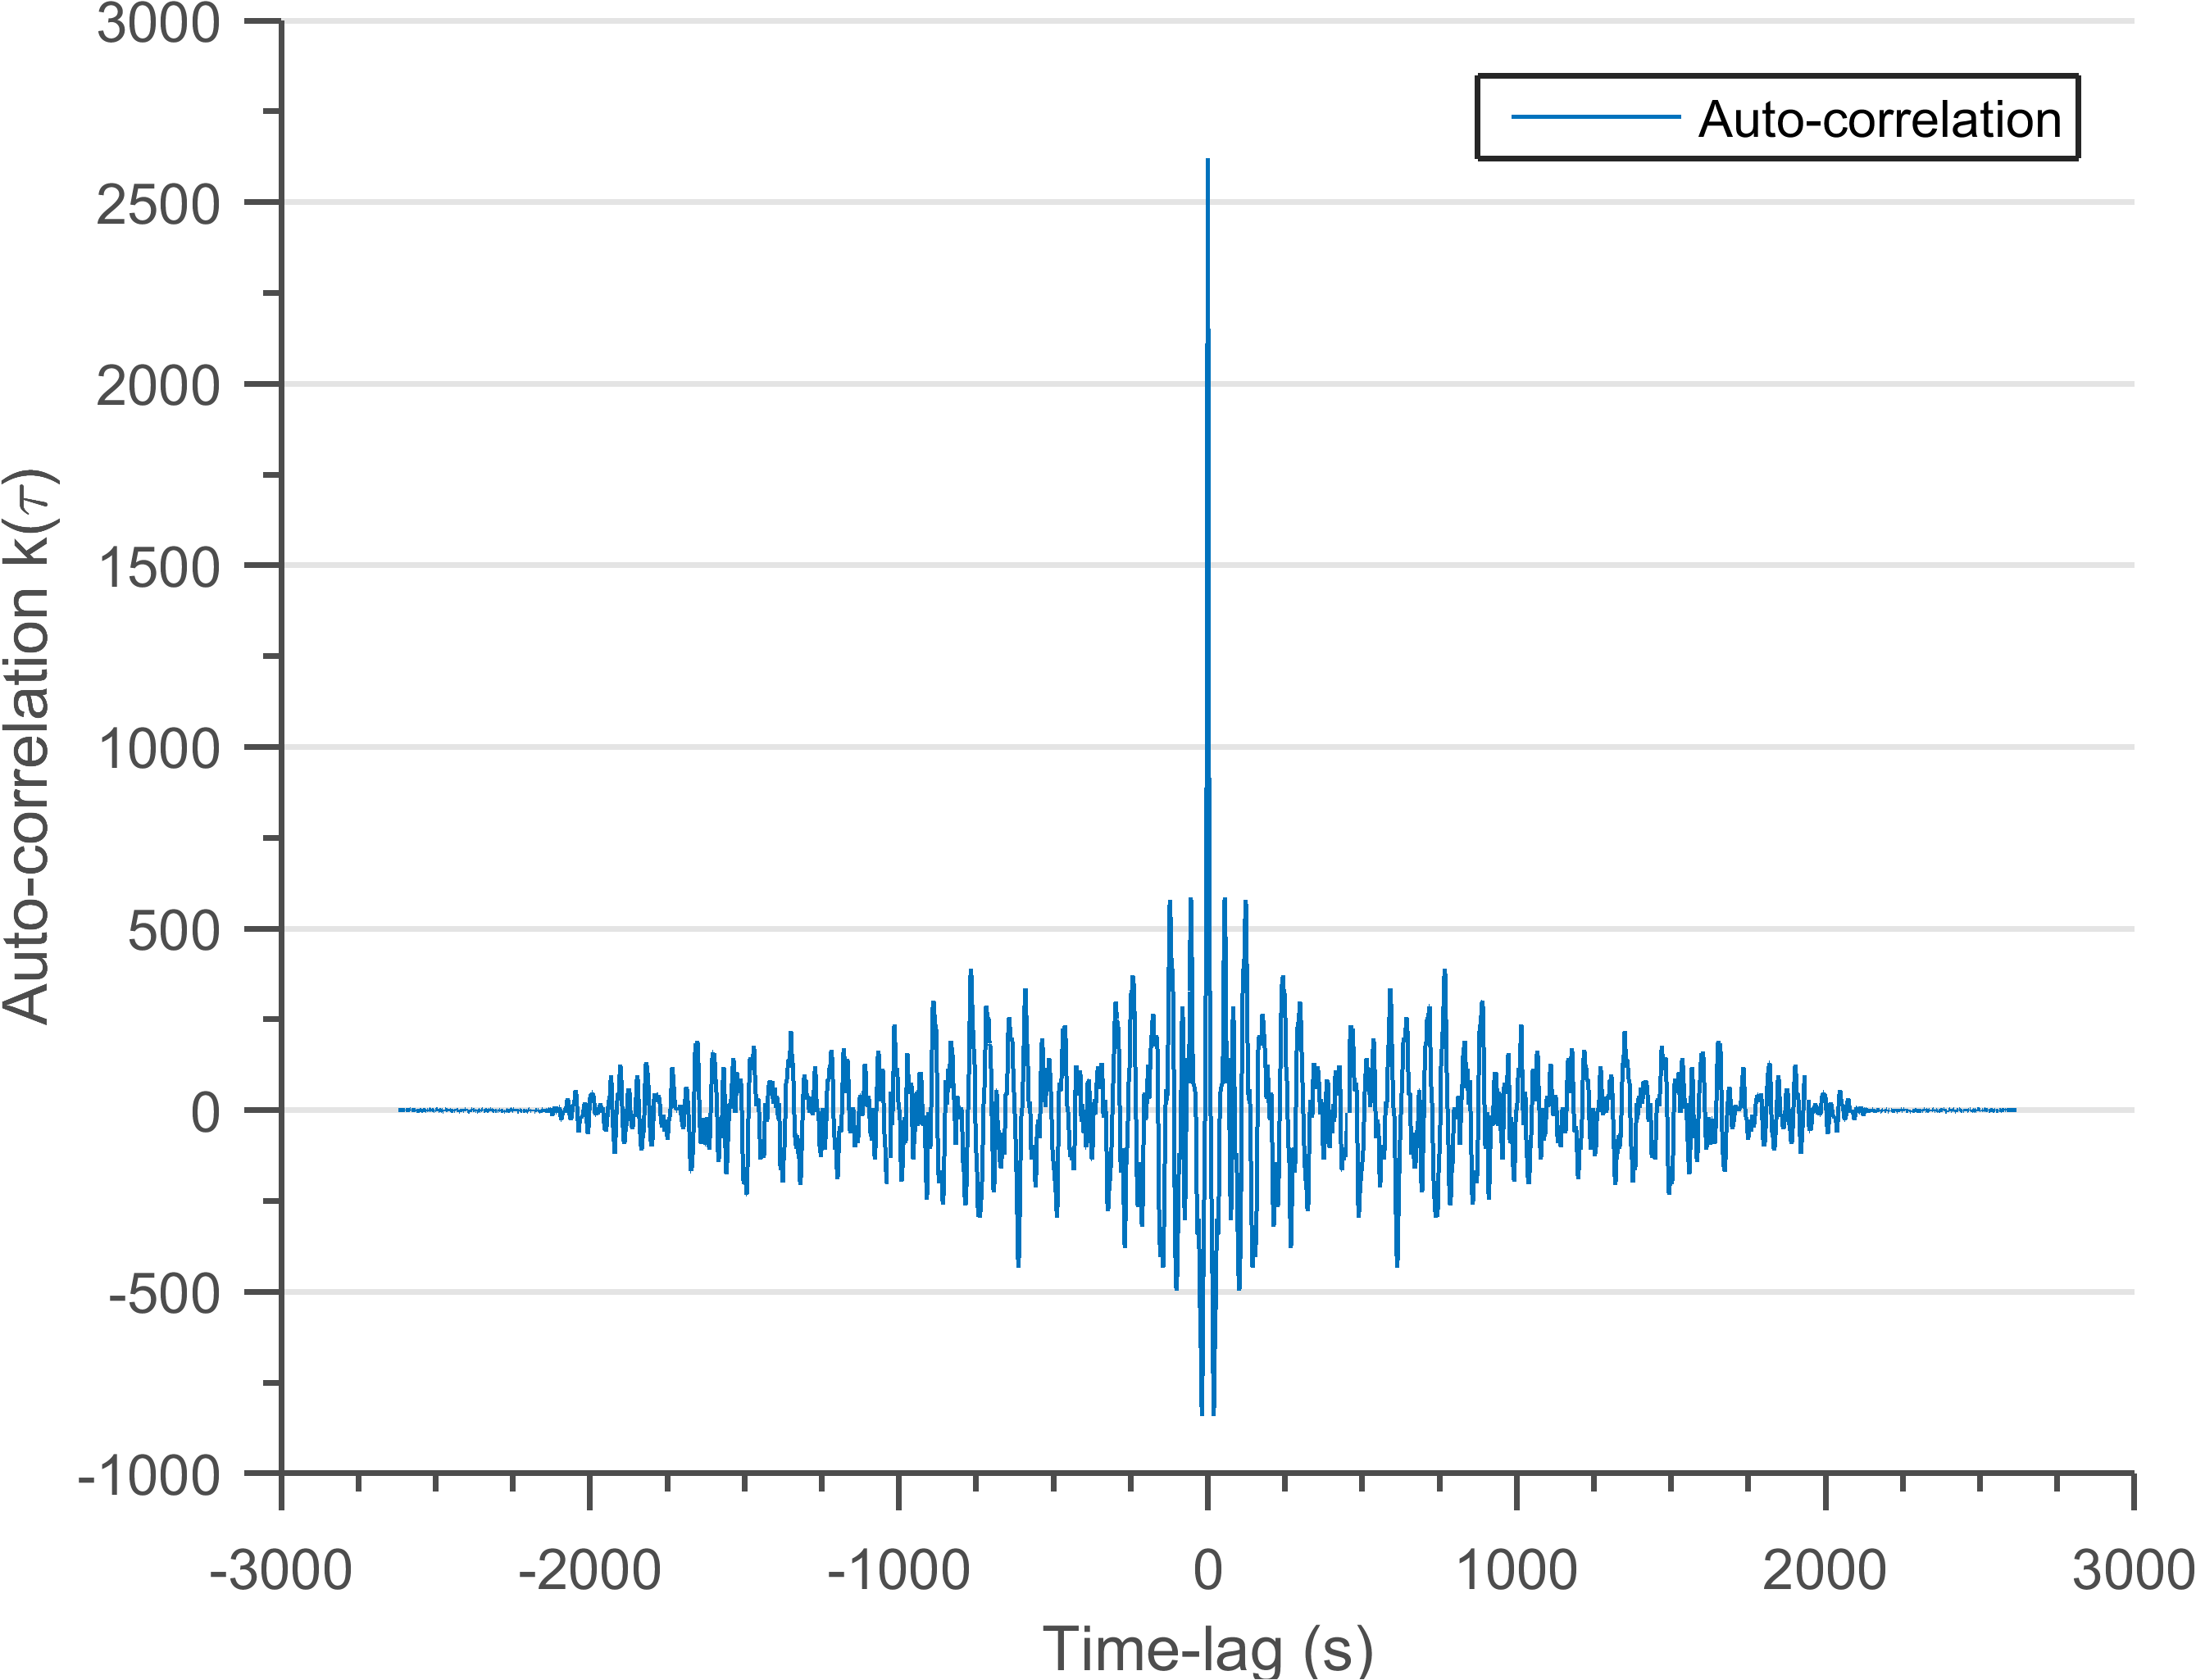
\includegraphics[width=0.3\textwidth]{images/autocorrelationOutput}\label{subfig:autocorrelationOutput}}\quad
  \subfigure[Power spectrum density \(S(s)\) of the output fig: \ref{subfig:randomOutput}]
  {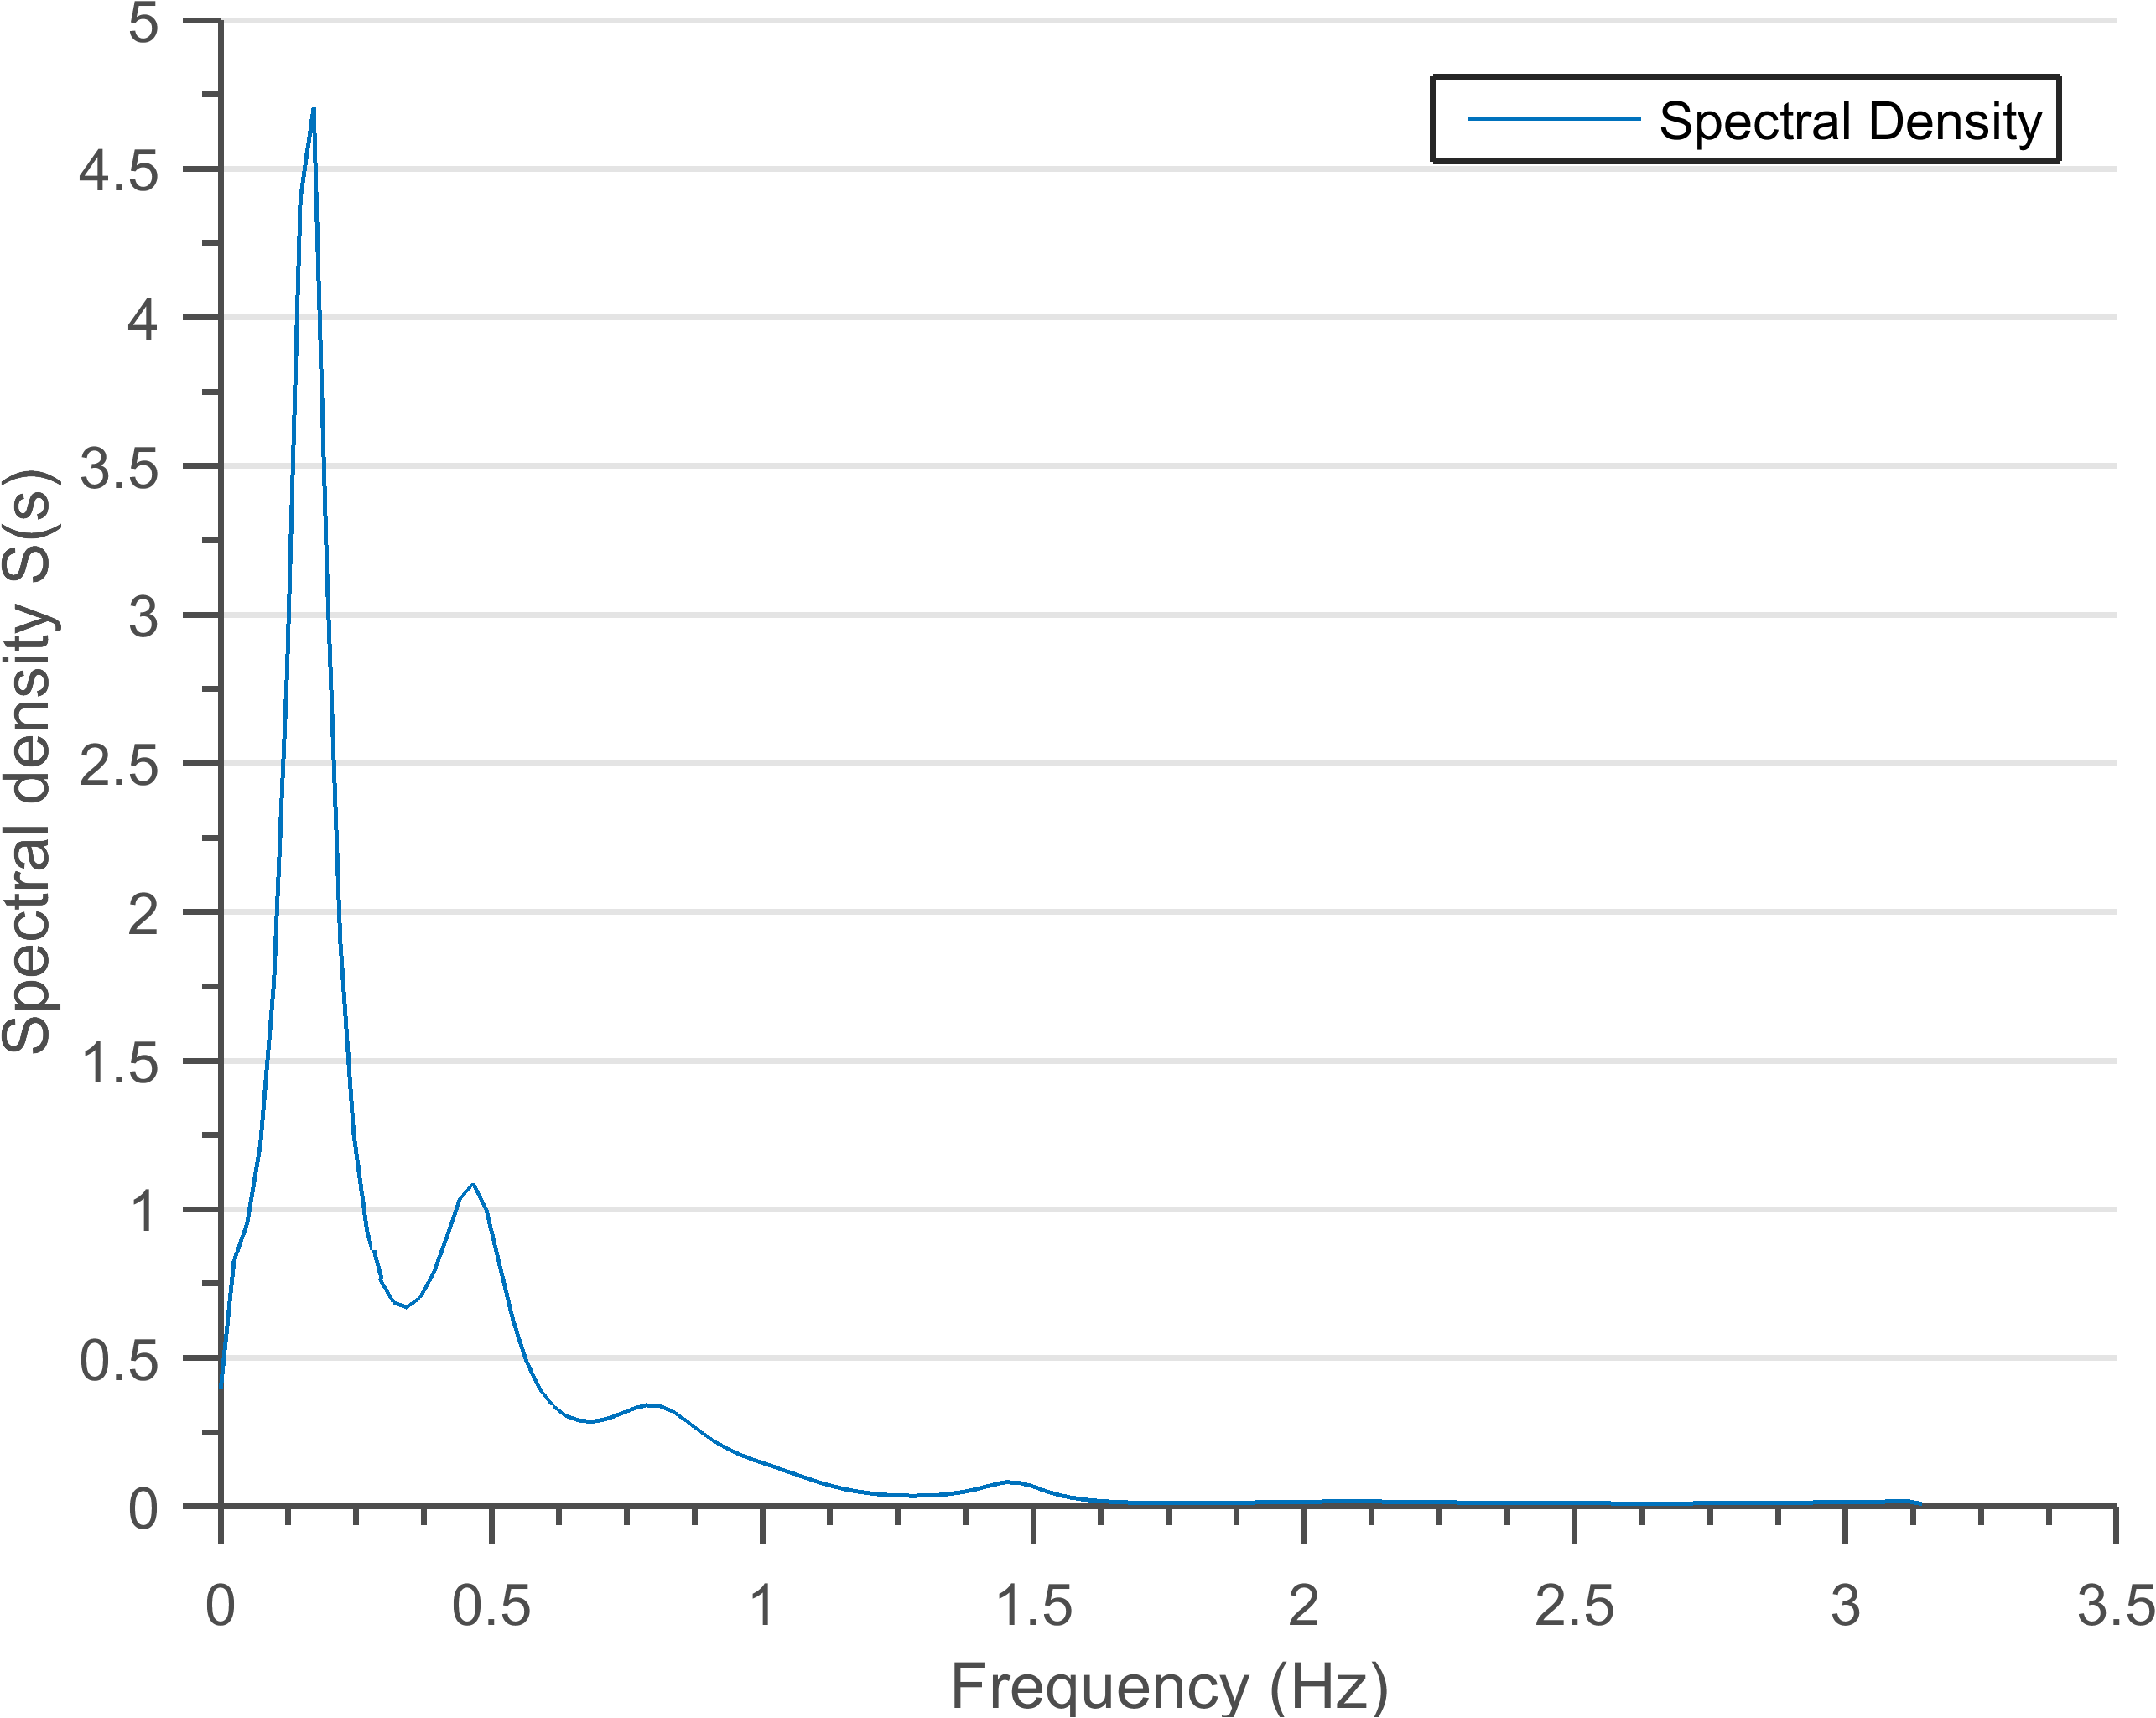
\includegraphics[width=0.3\textwidth]{images/psdOutput}\label{subfig:psdOutput}}
  
  \caption{Different types of measurements for estimation of Modal parameters in OMA}
\end{figure*}

\indent If we assume the measurement \(x(t)\) to be a stationary random process, then according to bochner's theorem \cite{bochner2016lectures} the spectral density or power spectrum \(S(s)\) can be represented as equation \ref{eq:spectralDensity}.

\begin{equation}\label{eq:spectralDensity}
    S(s) = \int k(\tau)exp(-2 \pi i s^{T} \tau )d\tau 
\end{equation}
Here, \(S(s)\) is the power spectrum for the measurement \(x(t)\), where \(s\) lies in the frequency-damping plane. Figure \ref{subfig:psdOutput} shows the power spectrum calculated for the measurement \(x(t)\) shown in figure \ref{subfig:randomOutput}. 

Initially the Peak Picking technique (PP) \cite{gade2005frequency} was used in the frequency-domain to identify modal frequencies and shapes. The PP technique is a very easy way to identify modes but becomes inefficient for complex structures \cite{zhang2004overview}. This gave rise to the Frequency Domain Decomposition (FDD) \cite{brincker2000modal} where modal frequency are denoted as the eigenvalues of spectral density matrix equation \ref{eq:FDD}.

Majority of frequency-domain algorithms in EMA fit a Rational Fractional Polynomial (RFP) \cite{richardson1982parameter} in the frequency domain for modal identification \cite{allemang1998unified} \cite{chauhan2007unified}. The Rational Fractional Polynomial equation \ref{eq:RFP} form can be derived if we assume the system to be second order differential equation \ref{eq:secondOrderSystem}.
\begin{table*}[t]
  \centering
  \setlength\extrarowheight{8pt}
\begin{tabular}{ |c|c|c| } 
  \hline
  Measurement; eg. figure \ref{subfig:randomOutput} & Auto-correlation; eg. figure \ref{subfig:autocorrelationOutput} & Power Spectrum; eg. figure \ref{subfig:psdOutput} \\
  \hline
  $x(t)$ & $k(\tau) = \int x(t)x(t-\tau)dt$ &  $S(s) = \int k(\tau)exp(-2 \pi i s^{T} \tau )d\tau$\\
  \hline \hline
  \multicolumn{3}{|c|}{Assumption: Second Order Differential}\\
  \hline
   & $k(\tau) = \sum A_{i}exp(-\lambda_{i}\tau)sin(B_{i}\tau)$ & $S(j\omega) = \frac{\sum a_{k}(j\omega)^{k}}{\sum b_{l}(j\omega)^{l}}$\\
   \hline \hline
   \multicolumn{3}{|c|}{Assumption: Gaussian Mixture Model}\\
   \hline
   $x(t) = GP(0 , cov_{SM})$ 
   & $k(\tau) = \sum w_{i} cos(2\pi\mu_{i}\tau) exp\{-2\pi^{2}\sigma_{i}^{2}\tau^{2}\}$ 
   & $S(s) = \sum w_{i}  \frac{1}{\sqrt{2\pi\sigma_{i}^{2}}}exp\{\frac{1}{2\sigma_{i}^{2}}(s-\mu_{i})^{2}\} $\\
   \hline
\end{tabular}
  \caption{Comparison of fitting functions}
  \label{tab:comparisonOfFittingFunctions}
\end{table*}

Moreover, if we assume that \(x(t)\) is a zero-mean gaussian process, then we can transform GMM in frequency-domain to time-domain. The equation \ref{eq:GMM} and equation \ref{eq:timeDomainGMM} are equivalent to fitting a zero-mean gaussian process with a spectral mixture covariance function \cite{wilson2013gaussian}.

\begin{equation}\label{eq:dataDomainGMM}
    x(t) = GP(0 , cov_{SM}(t, t'))
\end{equation}

Here, \(GP\) denotes a gaussian process \cite{Rasmussen2005}, while \(cov_{SM}\) represents a spectral mixture covariance function which resembles equation \ref{eq:timeDomainGMM} \cite{wilson2013gaussian}. 

We would like to emphasize that keeping the computational complexities aside, fitting a spectral mixture gaussian process in time-domain equation \ref{eq:GMM}, fitting equation \ref{eq:timeDomainGMM} for covariance-driven modal identification and fitting a GMM equation \ref{eq:GMM} in the frequency-domain are equivalent. In fact the initial idea of this paper was to fit a Gaussian Process (GP) in the data domain, but GP's are computationally heavy and we achieved a good accuracy by fitting the GMM in frequency domain. Refer to table \ref{tab:comparisonOfFittingFunctions} for a more comprehensive view at various fitting functions.

\begin{figure*}[!ht]
  \centering
  \subfigure[Stabilization diagram with increasing number of gaussians $Q$, the dots denote the stabilized frequencies. We can observe that as the number of $Q$ increases the algorithm starts finding better and better modes.]
  {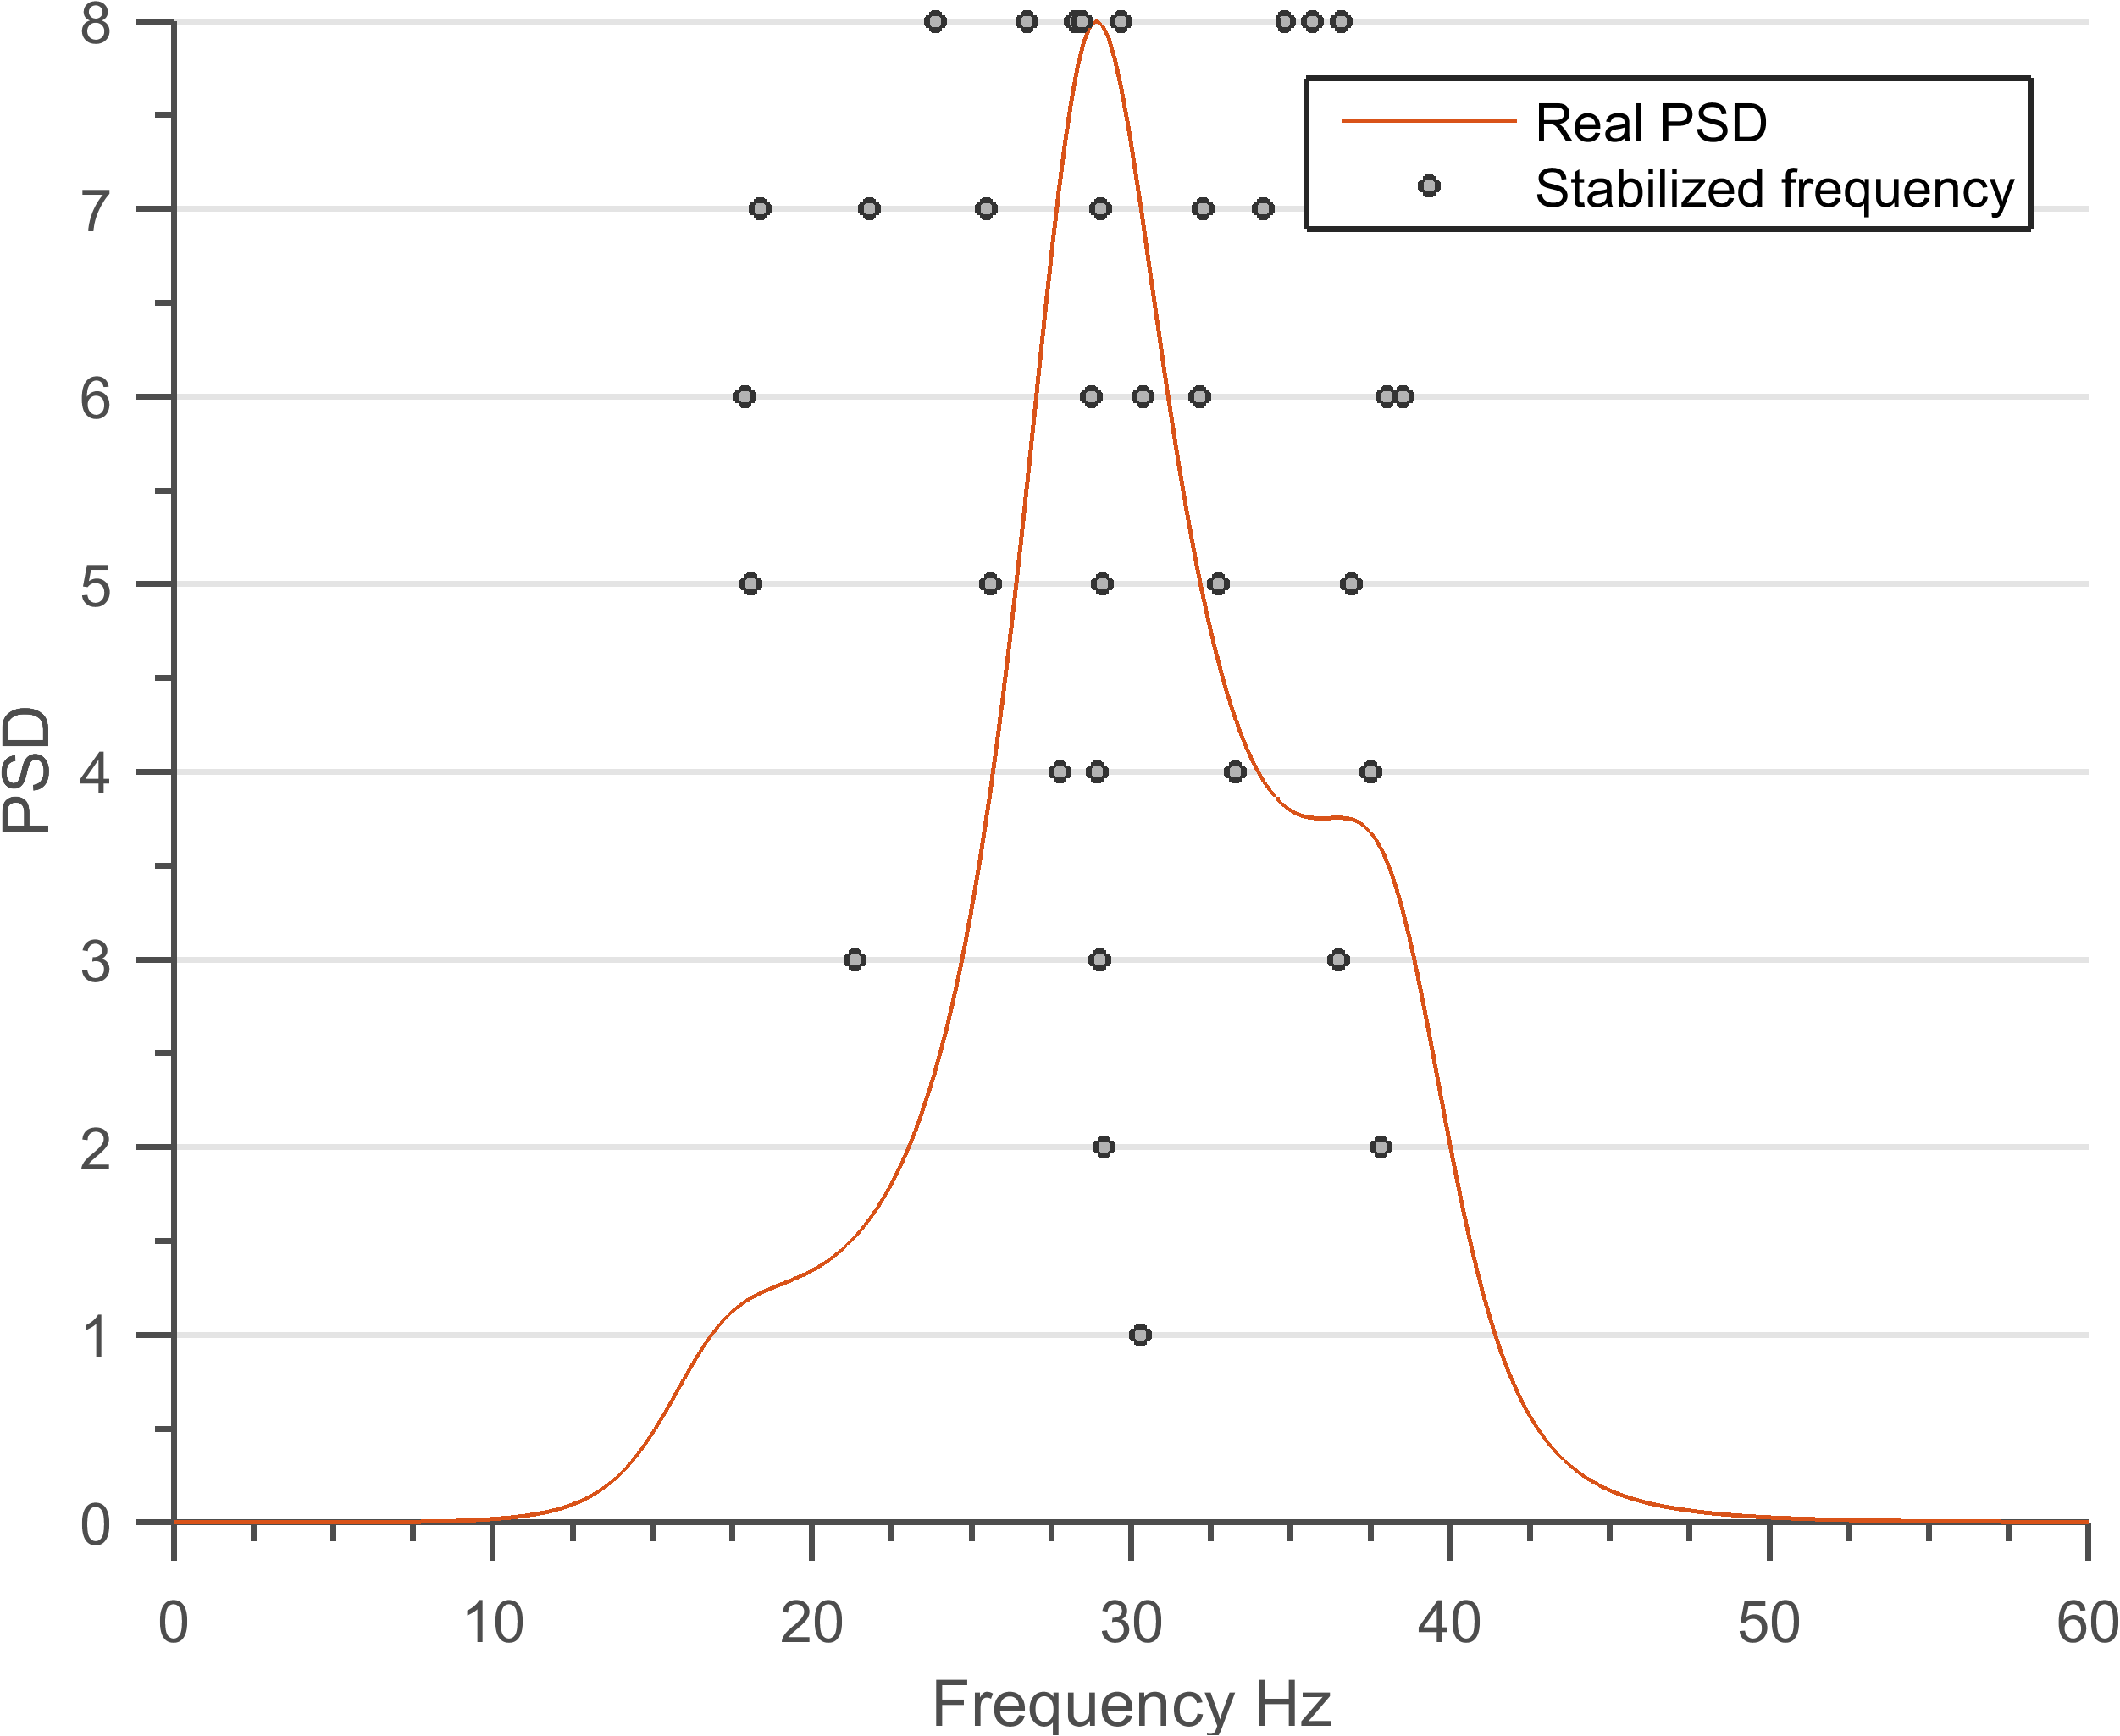
\includegraphics[width=0.3\textwidth]{images/stabilizationDiagram}\label{subfig:stabilizationDiagram}}\quad
    \subfigure[The BIC criterion with increasing number of gaussian's $Q$. We can see that that the BIC is minimum for $Q=6$ and hence if we add anymore gaussian's for our dataset we will be performing over-fitting]
  {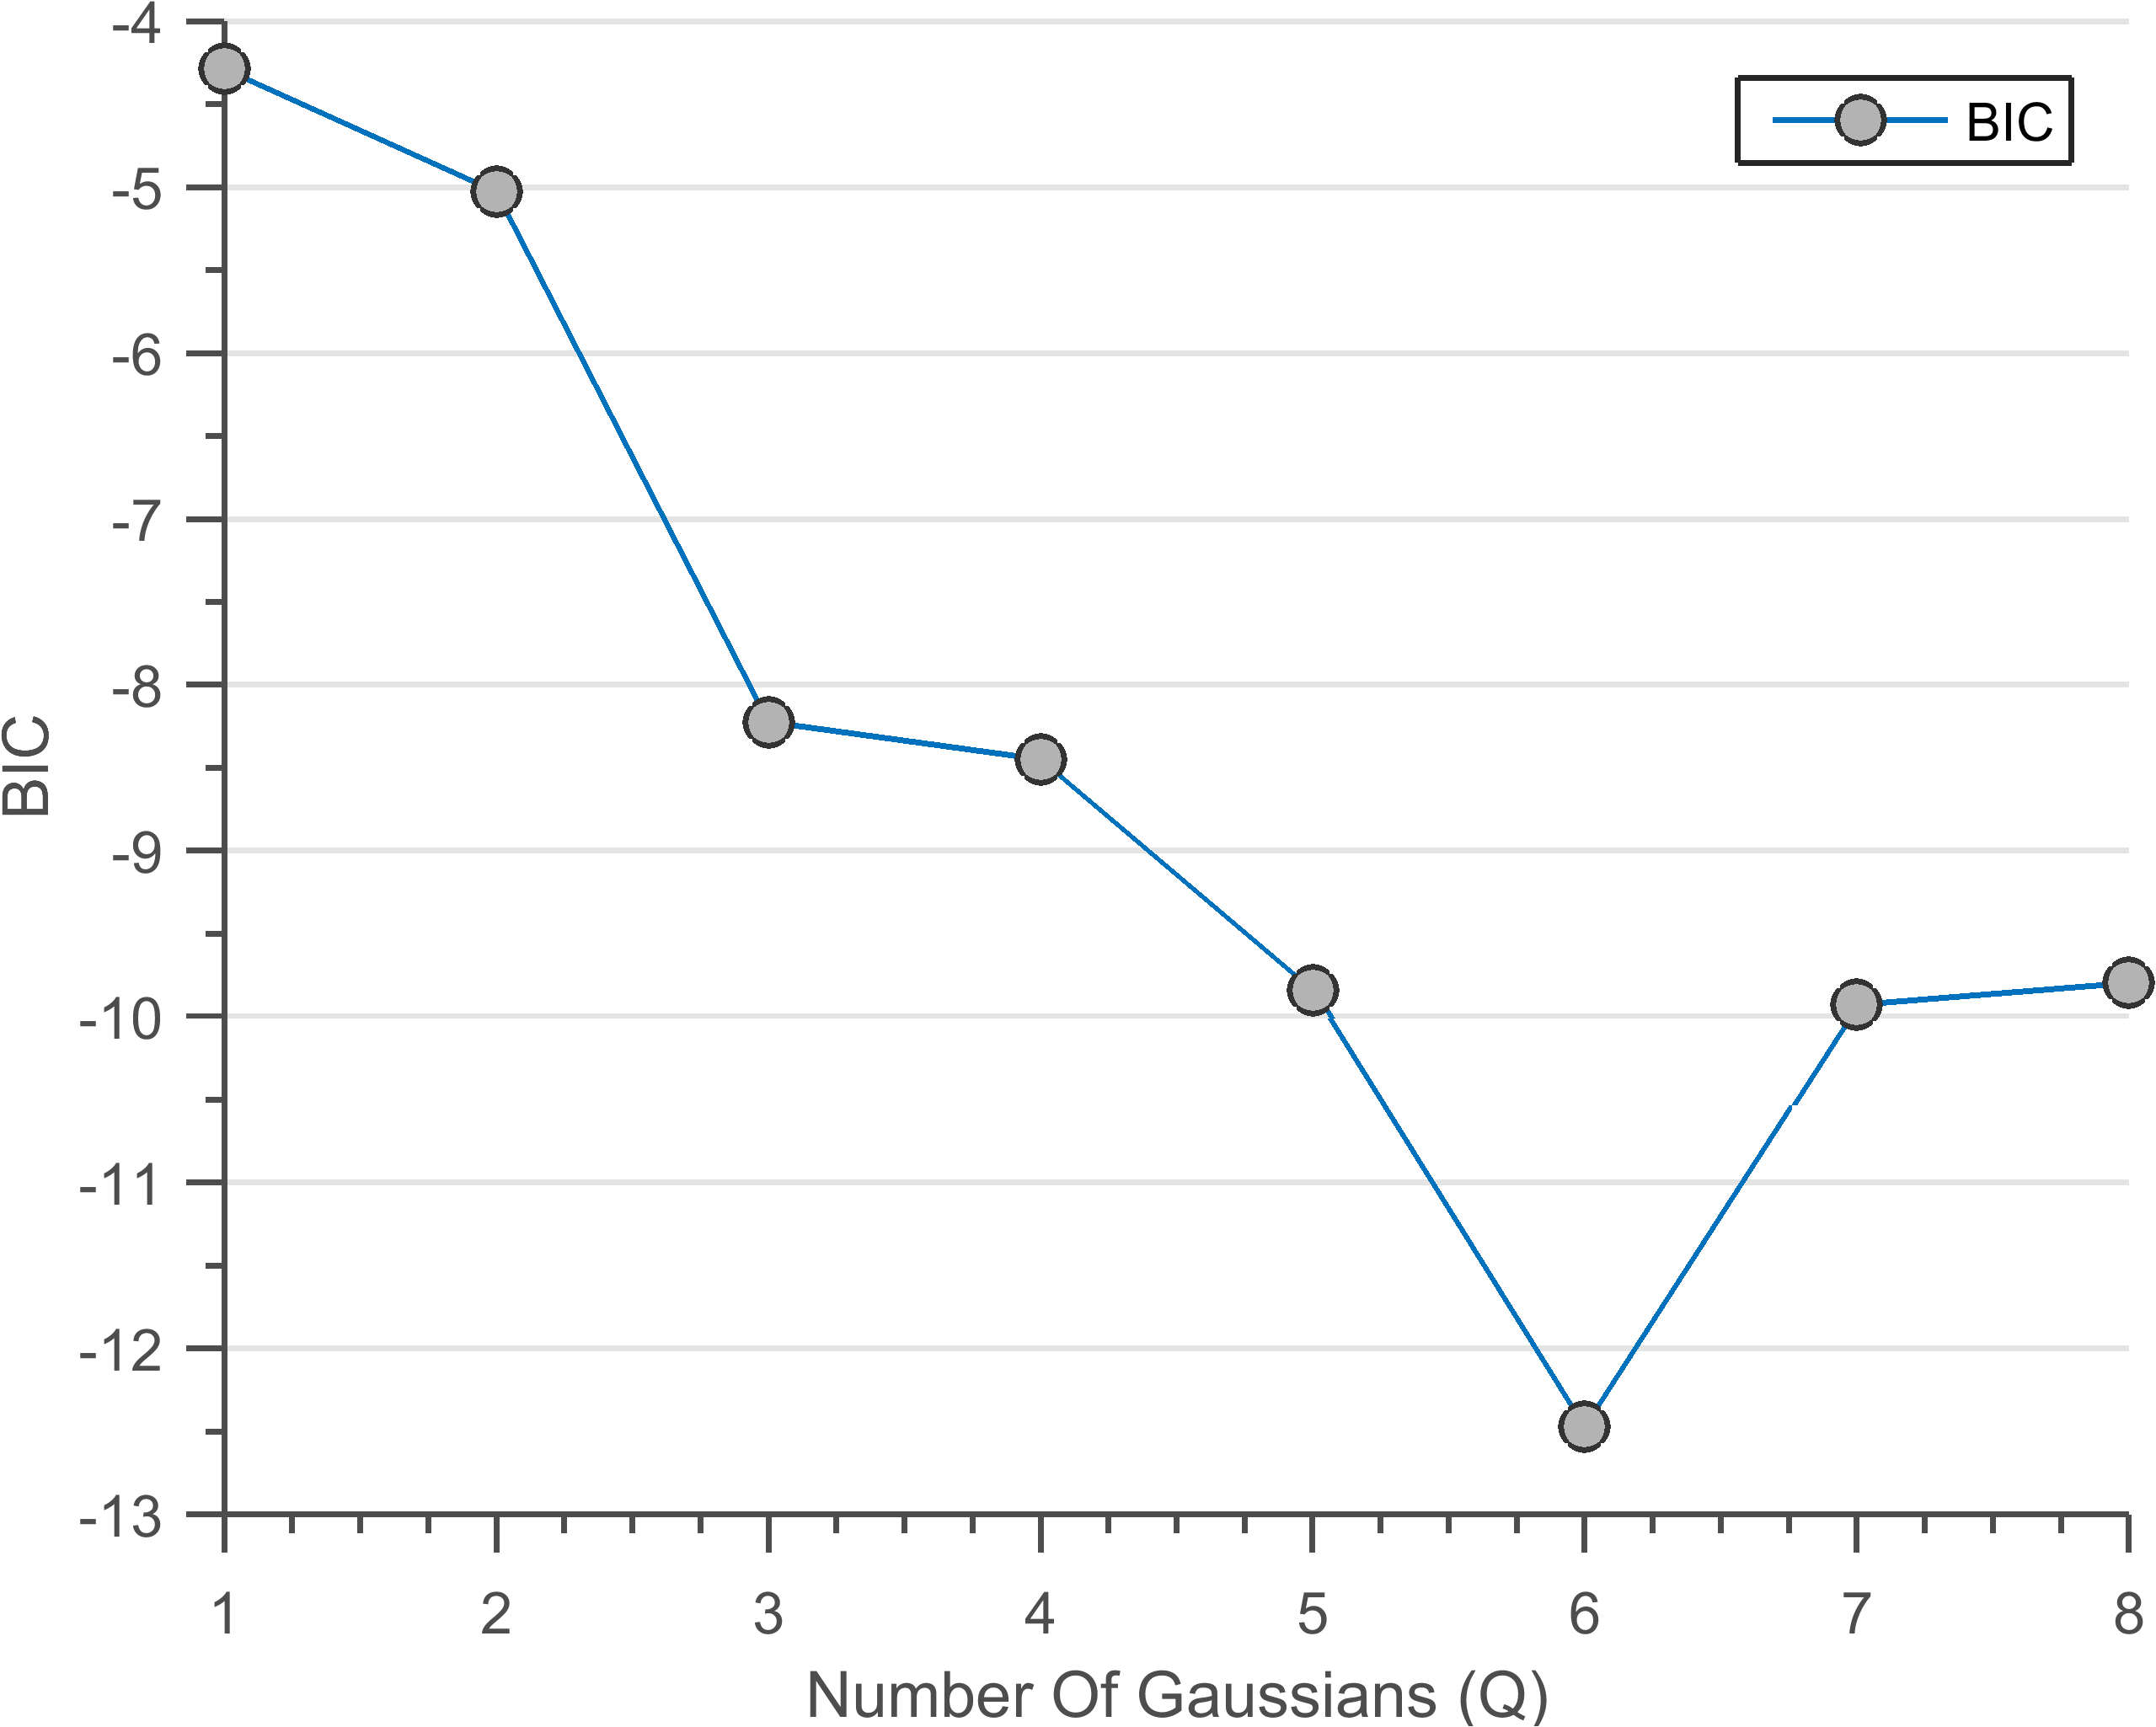
\includegraphics[width=0.3\textwidth]{images/bicVsQ}\label{subfig:bicVsQ}}\quad
  \subfigure[Distribution of  gaussians for $Q=6$. We can see that the three modal frequencies have majority of the participation in representing the spectral density.]
  {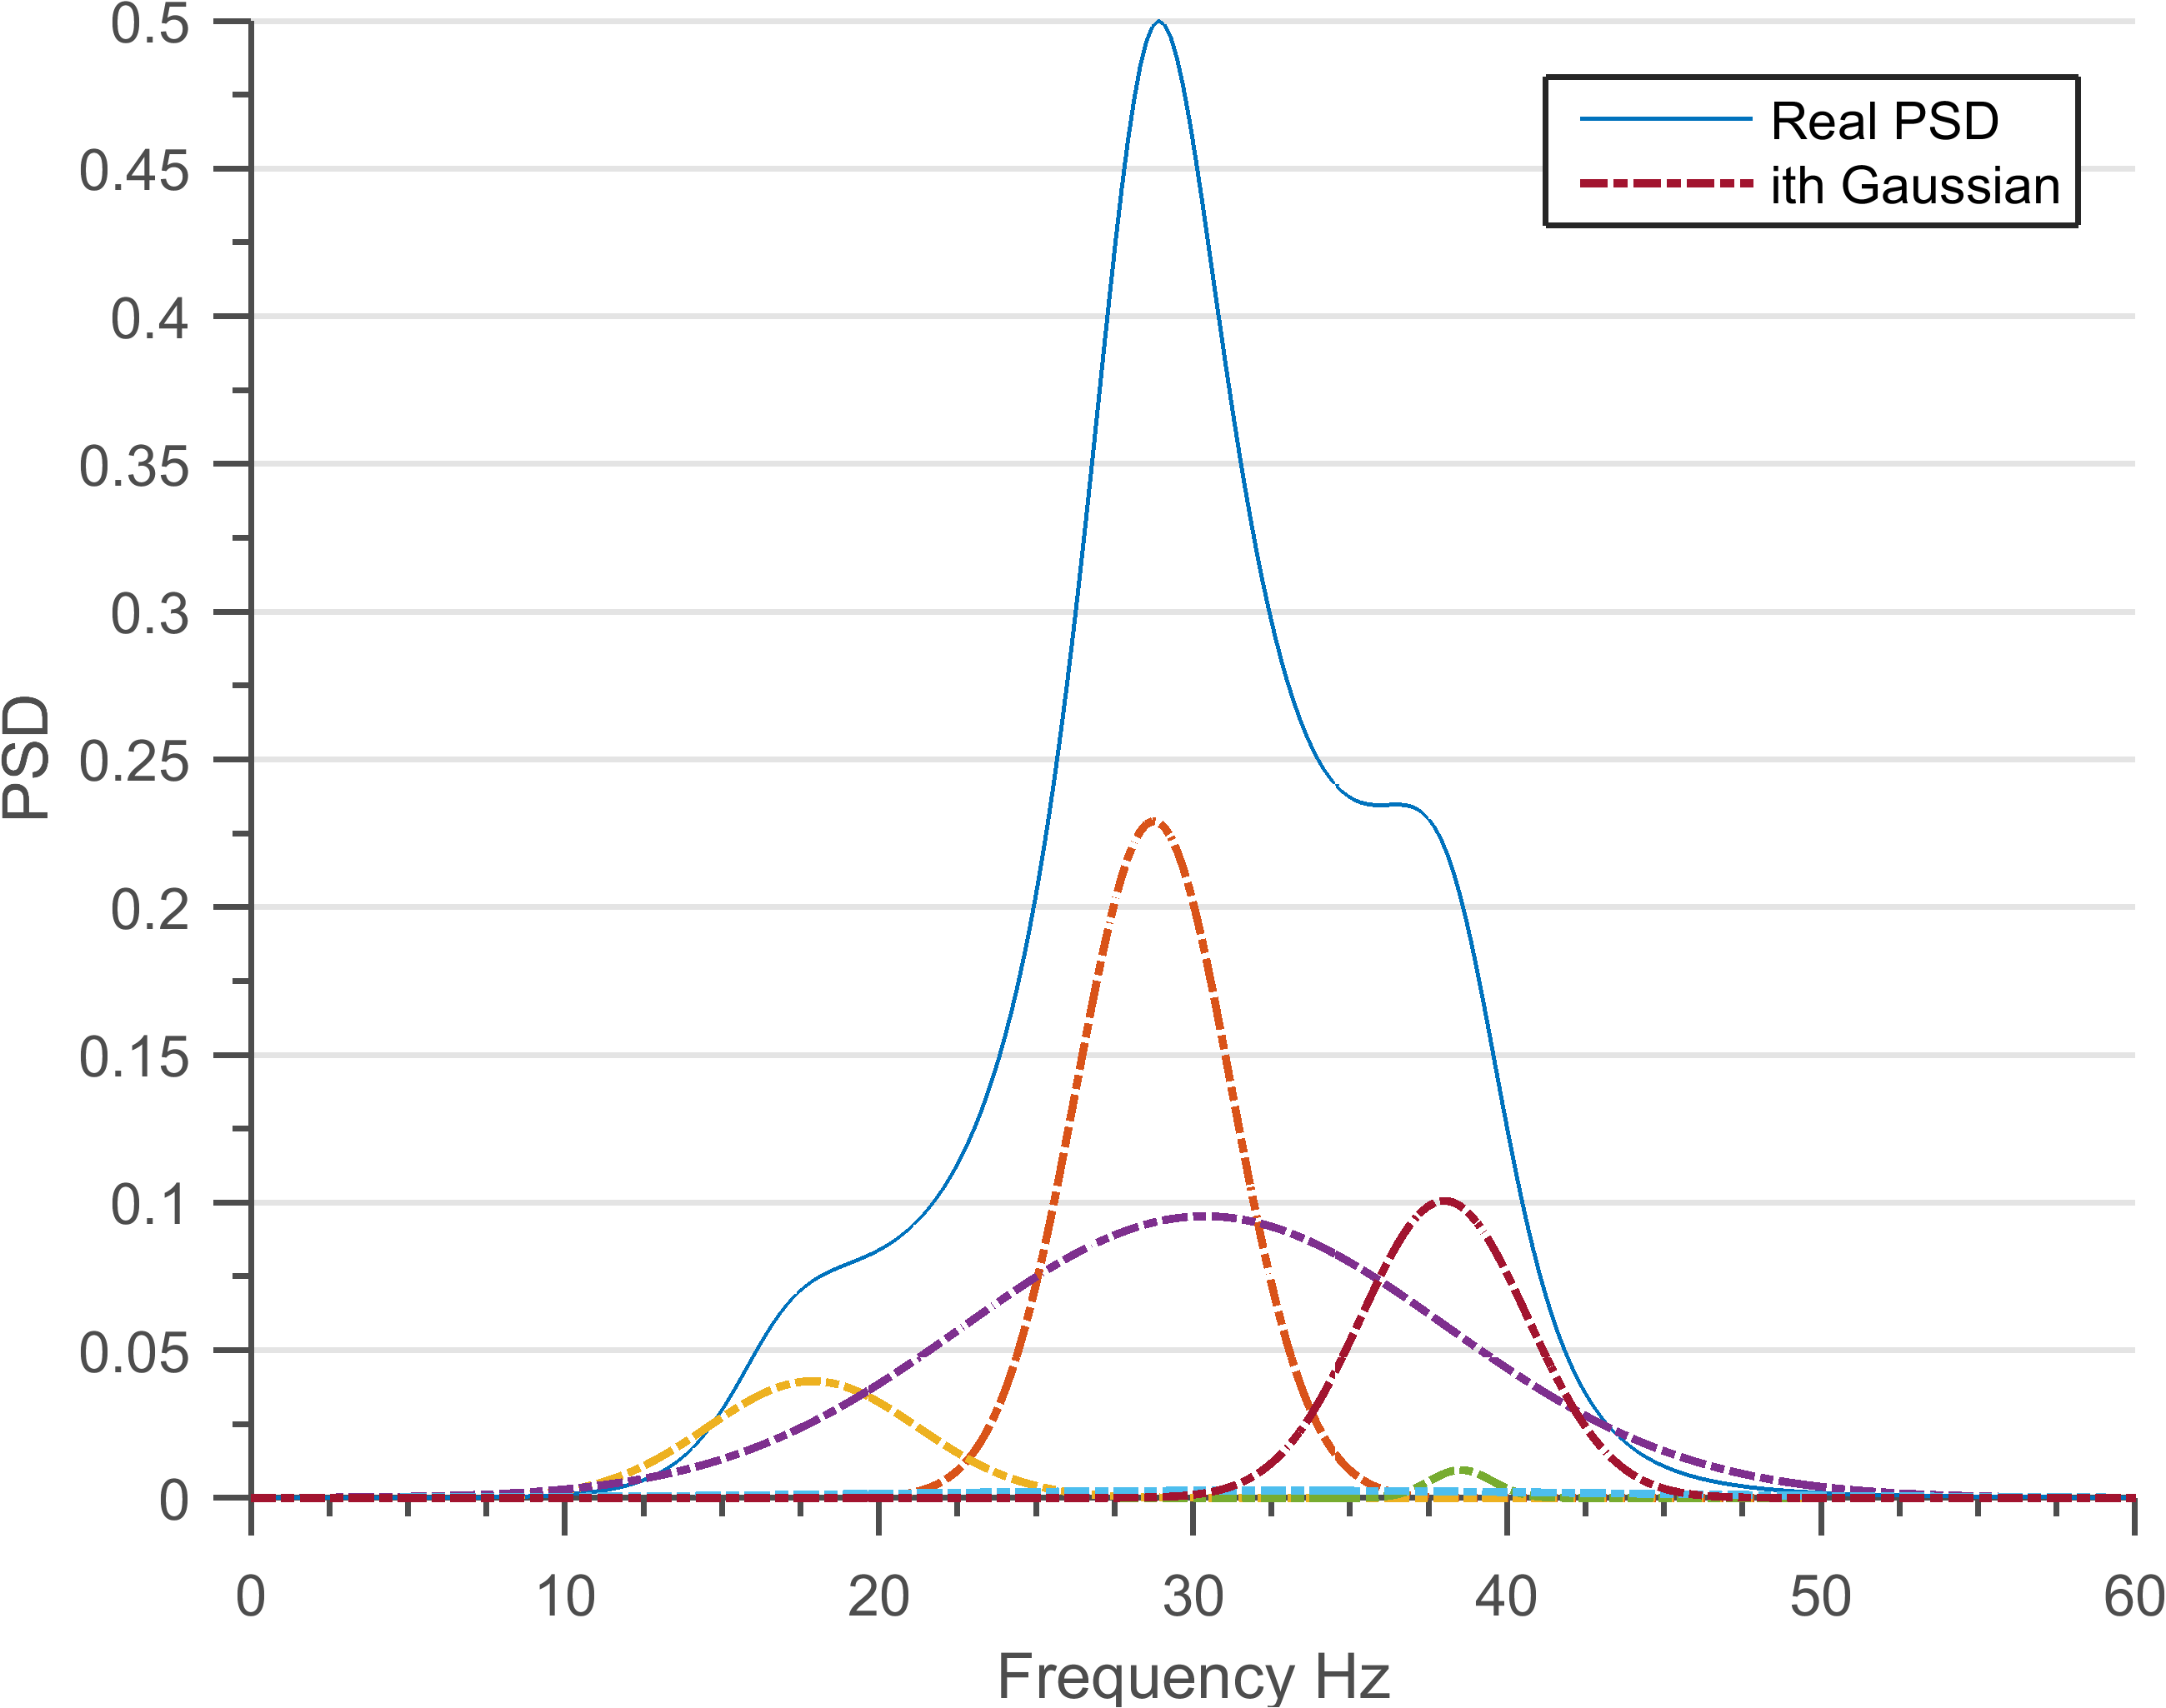
\includegraphics[width=0.3\textwidth]{images/distriButionOfGaussians}\label{subfig:distriButionOfGaussians}}

Figure \ref{subfig:stabilizationDiagram} shows the stabilization diagram with increasing number of gaussians $Q$. We can observe that as the number of $Q$ increases the algorithm starts finding better and better modes. We can also observe that there are three modes which start stabilizing from $Q=5$. The, figure \ref{subfig:bicVsQ} shows the BIC criterion with increasing number of gaussian's $Q$. We can see that that the BIC is minimum for $Q=6$ and hence if we add anymore gaussian's for our dataset we will be performing over-fitting.

Figure \ref{subfig:distriButionOfGaussians} shows the $6$ constituent gaussians which represent the $Q=6$ case. The three principal peaks represent the modal frequencies of the system, these correspond to the stabilized frequencies from figure \ref{subfig:stabilizationDiagram}. The remaining three peaks are there to compensate for the spectral density not explained by the three principal peaks. 

In the current setting of the GMM model we only propose a quick and easy way to identify the most important frequencies of a structural system. Neither the mode shapes nor the damping ratios are estimated in the current format. As can be observed from figure \ref{subfig:distriButionOfGaussians} the mode shapes are not only dependent on the principal gaussian's but also on the neighbouring gaussian's. Since some part of the spectral density is defined by non-stabilized gaussian's, in future we would like to derive a method to estimate mode-shape and damping ratio such that the contributions of neighbouring gaussian's are also taken into account.
  
  \caption{Results of applying GMM on a Spectral density}
\end{figure*}

In this paper we have proposed to identify model frequencies of a system by curve-fitting a mixture of gaussians in the frequency domain. While the common assumption that the structure can be modelled as a MDOF second order differential system causes stability issues in presence of non-linear systems. The GMM model is mathematically stable, gives results in seconds and can fit a function upto arbitrary accuracy. Moreover we introduce the BIC to identify the optimum number of gaussians and perform a trade-off between accuracy of fit and over-fitting. 

Without doubt this is very nascent stage of application of GMM for system identification and there remains problems such as identification of mode-shape and damping ratio in this algorithm. We wish to tackle these problems in the future. We also wish to apply the algorithm on a real world dataset and compare with respect to other time domain and frequency domain techniques.


%%% Local Variables: 
%%% mode: latex
%%% TeX-master: "isae-report-template"
%%% End: 